% Created 2025-04-29 Tue 19:09
% Intended LaTeX compiler: pdflatex
\documentclass[11pt]{article}
\usepackage[utf8]{inputenc}
\usepackage[T1]{fontenc}
\usepackage{graphicx}
\usepackage{longtable}
\usepackage{wrapfig}
\usepackage{rotating}
\usepackage[normalem]{ulem}
\usepackage{amsmath}
\usepackage{amssymb}
\usepackage{capt-of}
\usepackage{hyperref}
\usepackage{minted}
\usepackage{siunitx}
\usepackage{array}
\setlength{\parindent}{0em}
\author{Hankertrix}
\date{\today}
\title{MA2012 Introduction to Mechatronics System Design Notes}
\hypersetup{
 pdfauthor={Hankertrix},
 pdftitle={MA2012 Introduction to Mechatronics System Design Notes},
 pdfkeywords={},
 pdfsubject={},
 pdfcreator={Emacs 30.1 (Org mode 9.7.11)}, 
 pdflang={English}}
\begin{document}

\maketitle
\setcounter{tocdepth}{2}
\tableofcontents \clearpage\section{Definitions}
\label{sec:org6a5a441}

\subsection{Mechatronics}
\label{sec:org0a997cb}
\begin{itemize}
\item A combination of the word "Mecha-nical" and "Elec-tronics". It is a termed coined in Japan in the 1960s.
\item It is an interdisciplinary field of engineering dealing with the design of products whose function relies on the integration of mechanical and electronic components coordinated by a control architecture.
\end{itemize}
\subsection{System}
\label{sec:org11e1205}
A combination of related parts combined into a complex whole.
\subsection{System science}
\label{sec:orgfe3e36e}
An interdisciplinary field of science that studies the nature of complex systems.
\subsection{System engineering}
\label{sec:org06c68a1}
An interdisciplinary field of engineering that focuses on how complex systems should be designed, engineered and managed.
\subsection{Measurement system}
\label{sec:orgb633593}
A system that presents an observer with a numerical value that represents the state or change of a variable of a process, machine or system being measured.
\begin{center}
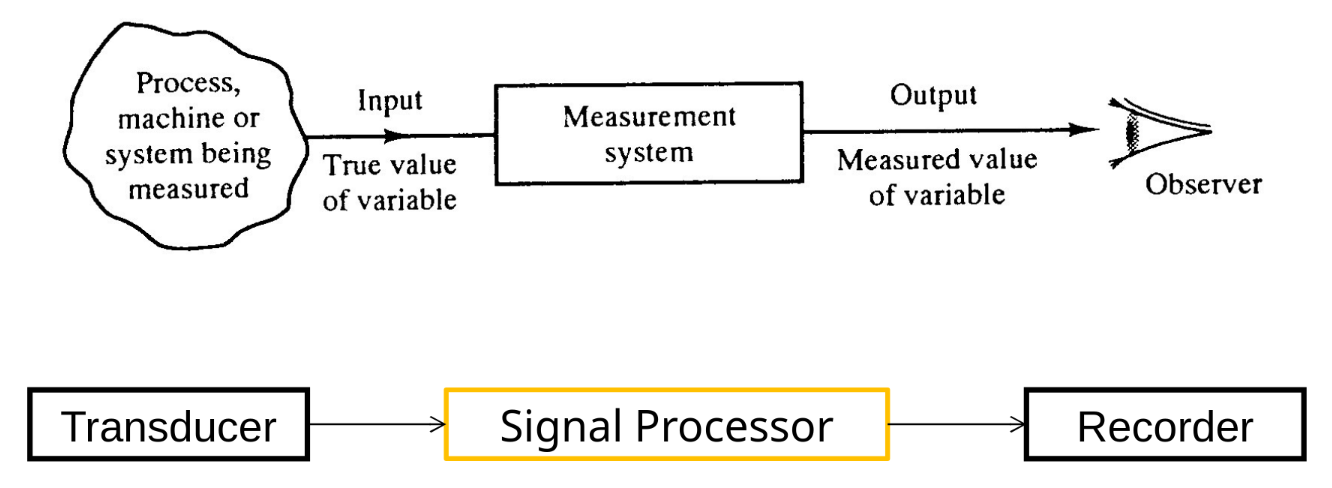
\includegraphics[width=.9\linewidth]{./images/measurement-system.png}
\end{center}
\subsection{Actuation system}
\label{sec:org3e09752}
A system that converts one form of energy (e.g. electrical, chemical, etc.) to another to perform mechanical work (e.g. movement, heat, etc.).
\begin{center}
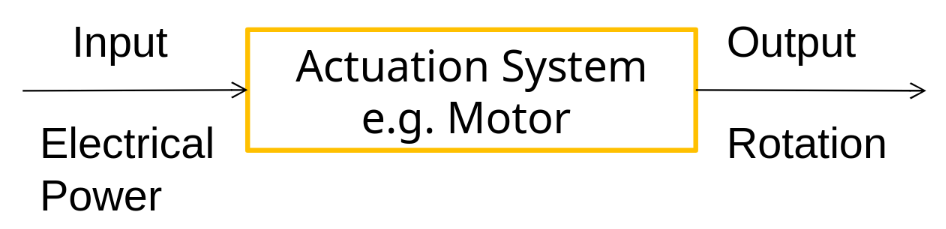
\includegraphics[width=.9\linewidth]{./images/actuation-system.png}
\end{center}
\subsection{Control system}
\label{sec:org28db679}
A system to modify one or more measurable parameters of a plant or process to achieve desired outputs. For example, a central heating system:
\begin{itemize}
\item Input: Electrical power
\item Actuation system: Heating coil and blower
\item Plant: Environment or room
\item Measurement system: Temperature sensor
\item Output: Desired temperature
\end{itemize}
\subsection{Microprocessor (MPU)}
\label{sec:org82c3bbb}
A microprocessor refers to the Central Processing Unit (CPU) on a single integrated-circuit (IC) chip.
\subsection{Microcomputer}
\label{sec:org44afd62}
A microcomputer refers to the MPU combined with the memory (RAM) and input and output unit (I/O unit).
\subsection{Microcontroller (MCU)}
\label{sec:orge841101}
A microcontroller (MCU) refers to the microcomputer (CPU + Memory + I/O) in a single integrated-circuit (IC) chip.
\subsection{Embedded systems}
\label{sec:org081b0ab}
Embedded systems are microcontrollers for a single purpose (not single function).
\subsubsection{Examples}
\label{sec:org54cb932}
\begin{itemize}
\item Consumer products: Mobile phones, washers, fridge, air-conditioner, etc.
\item Healthcare products: Treadmills, blood glucose metre, etc.
\item Automobile system controller
\item And much more\ldots{}
\end{itemize}
\subsubsection{Advantages}
\label{sec:orge447be9}
Embedded systems are cheap, small and have low power consumption.
\subsubsection{Disadvantages}
\label{sec:orgd690330}
Embedded systems are inflexible and have limited or even no expandability.
\subsection{General purpose computers}
\label{sec:org8132c2f}
General purpose computers are computers that are for general use and can do a wide variety of tasks. They are outnumbered by embedded systems in a ratio of \(\textgreater 100:1\)
\subsubsection{Examples}
\label{sec:orgc9d6123}
Personal computer (PC), Macintosh, Workstations, Personal Digital Assistant (PDA), Smartphone, etc.
\subsubsection{Advantages}
\label{sec:orgfcec580}
\begin{itemize}
\item Flexibility, as general purpose computers are capable of running many kinds of software and interface with lots of devices.
\item Expandability and scalability, as the software and the hardware of general purpose computers are upgradeable.
\end{itemize}
\subsubsection{Disadvantages}
\label{sec:orgd9c9885}
\begin{itemize}
\item Complexity, to cater for flexibility and expandability
\item Cost, as general purpose computers cost from \$100 to upwards of \(\$\)10,000
\item High power consumption
\end{itemize}
\subsection{Central Processing Unit (CPU)}
\label{sec:org95d83dc}
\begin{itemize}
\item The CPU consists of the arithmetic and logic unit and the control unit
\item Arithmetic and Logic Unit (ALU)
\begin{itemize}
\item Arithmetic: \(+, -, \times, \div\), etc.
\item Logic: OR, AND, NOT, NOR, NAND, XOR, etc.
\item Result of ALU is usually stored in the accumulator register
\end{itemize}
\item Control Unit
\begin{itemize}
\item Directs the operation of all parts of a computer by providing timing and control signals
\item Fetches, decodes, and executes the instructions in memory.
\end{itemize}
\end{itemize}
\subsection{Memory}
\label{sec:org3d309ac}
\begin{itemize}
\item A memory cell is a device or circuit used to store a single bit ("1" or "0"), like flash file system (FFS), magnetic core memory, disks.
\item A memory word is a group of memory cells.
\item Internal memory, also known as main or working memory, is the highest speed memory.
\item Memory is used to store programs for sequenced execution.
\item Memory is also used to store data for output at required time.
\item Types of memory
\begin{itemize}
\item Random Access Memory (RAM)
\item Read-Only Memory (ROM)
\item Electrically Erasable Programmable Read-Only Memory (EEPROM)
\item Flash memory
\end{itemize}
\end{itemize}
\subsubsection{Random access memory (RAM)}
\label{sec:orga816f9c}
\begin{itemize}
\item Any memory device that can go directly to an address without having to sequence through other locations.
\item Random access memory is volatile, which means the data is lost when the system loses power.
\item Variables and I/O data are stored in random access memory when arithmetic and logic operations are performed on them.
\item The Arduino Uno has static random access memory with a capacity of \(\qty{2}{kB}\)
\end{itemize}
\subsubsection{Static RAM (SRAM)}
\label{sec:org6b44476}
\begin{itemize}
\item A semiconductor RAM device that consists essentially of flip-flop registers and the necessary circuitry for decoding.
\item Information will remain valid as long as power is on.
\item It has the advantages of fast access speed and simple circuitry.
\end{itemize}
\subsubsection{Dynamic RAM (DRAM)}
\label{sec:org200f029}
\begin{itemize}
\item Memory devices that store binary data by charging the gate capacitances of Metal Oxide Semiconductor (MOS) transistors.
\item Refreshing or periodically recharging (roughly ever \(\qty{4}{ms}\)) is required
\item It has the advantages of lower cost for higher memory density, as well as low power consumption.
\end{itemize}
\subsubsection{Synchronous dynamic RAM (SDRAM)}
\label{sec:org0aae032}
\begin{itemize}
\item Synchronous dynamic RAM is DRAM which is synchronous with the system bus.
\item Use DRAM is when capacity and power consumption are valued more than access speed.
\end{itemize}
\subsubsection{Read-Only memory (ROM)}
\label{sec:org5a1340f}
\begin{itemize}
\item A semiconductor memory device designed primarily for having data read from them.
\item Data cannot be changed during operation.
\item The memory is non-volatile, which means the data persists even if the power is turned off.
\end{itemize}
\subsubsection{Erasable programmable ROM (EPROM)}
\label{sec:orgd874686}
\begin{itemize}
\item A semiconductor ROM device with which the user can erase and reprogram the contents of memory as many times as desired.
\item Exposure to UV lights erases information on the memory chip. The UV light sets all the cells to 1s.
\end{itemize}
\subsubsection{Electrically erasable programmable ROM (EEPROM)}
\label{sec:org1df0a7e}
\begin{itemize}
\item A semiconductor ROM device with which the user can erase and reprogram individual locations by the application of appropriate voltage levels and pulse durations.
\item The size of the EEPROM in the Arduino Uno is \(\qty{1}{kB}\).
\end{itemize}

 \newpage
\subsubsection{Flash memory}
\label{sec:org1f7eb9a}
\begin{itemize}
\item Flash memory is a type of EEPROM, which means it is non-volatile.
\item It is erasable and programmable, and it works with a block of data instead singular bits.
\item It also can be used as read-only memory (ROM), such as in flash Basic Input/Output System (BIOS), as a disk drive (USB drive, SD card, solid state drive, etc.) or random access memory (RAM), like flash RAM.
\item Flash memory has advantages over:
\begin{itemize}
\item EEPROM in versatility, as it can be used as RAM instead of just ROM
\item RAM in being non-volatile, as it can persist data even when the device is powered off, and it is also as fast as dynamic RAM (DRAM).
\item Disk drive in speed, as it has no moving parts, being a solid state drive.
\end{itemize}
\item The Arduino Uno contains \(\qty{32}{kB}\) of flash memory.
\end{itemize}
\subsection{Microprogram}
\label{sec:org188fc57}
\begin{itemize}
\item A collection of instructions that control the timing and control logic of all components of the microprocessor.
\item It is built into the microprocessor by the chipmaker and cannot be modified by programmers.
\end{itemize}
\subsection{Firmware}
\label{sec:org286ea93}
\begin{itemize}
\item Firmware is software programmed into the Read-Only Memory (ROM) of a microprocessor for the execution of functions of a device.
\item Programmed by device manufacturer and cannot be modified by users.
\end{itemize}
\subsection{Program (noun)}
\label{sec:org09869c4}
\begin{itemize}
\item A program is software loaded into the Random Access Memory (RAM) of a general purpose computer.
\item It is programmed by software developers (not necessarily device manufacturers) and cannot be modified by users.
\end{itemize}
\subsection{Program (verb)}
\label{sec:orga18a5d3}
Programming refers to a procedure of putting data into memory for non-volatile storage.
\subsection{Write}
\label{sec:orga58c39a}
Writing means an instruction that sends data to an address in RAM or external storage.
\subsection{System or frontside bus}
\label{sec:org042afb6}
\begin{itemize}
\item A system or frontside bus is the parallel conductor lines which connects the CPU to the other components.
\item A 64-bit processor needs the bus to be 64-bit wide, which is 1 bit of information per line.
\end{itemize}
\subsection{Double Data Rate (DDR)}
\label{sec:org5e4949c}
\begin{itemize}
\item Double data rate refers to data transfer at both the positive and negative transitions.
\item DDR\(n\), where \(n\) is a number, stands for DDR generation \(n\).
\end{itemize}
\subsubsection{Lower Power DDR (LPDDR)}
\label{sec:org62b2dcb}
Lower Power DDR is just DDR with lower power consumption to be used in mobile devices.
\subsubsection{Graphics DDR (GDDR)}
\label{sec:org1f71dbf}
Graphics DDR is just DDR for graphics cards.
\subsection{Bootloader program}
\label{sec:org0d31aad}
\begin{itemize}
\item A bootloader program is a program to "boot-up" or "bootstrap" the computer.
\item For a general purpose computer, it loads the operating system (Windows, iOS, Android, etc.) from hard drive or flash memory on to the RAM.
\item For the Arduino Uno, it does the following:
\begin{itemize}
\item It checks for new programming command from the serial connection to the PC.
\item If there is a new programming command, it downloads the new program from the PC into the Arduino.
\item Otherwise, it loads the latest programme stored in the flash memory.
\end{itemize}
\item The Arduino Uno bootloader program is activated when it is powered on or reset.
\end{itemize}
\subsection{Transducer}
\label{sec:org6c4fdd5}
A device which converts one form of energy into another.
\subsection{Sensor}
\label{sec:orgfb92f37}
\begin{itemize}
\item A sensor is a transducer which performs measurement.
\item It is a device which produces an output signal (typically electrical) for the purpose of sensing physical phenomena.
\end{itemize}
\subsection{Analogue quantity}
\label{sec:org111e096}
\begin{itemize}
\item An analogue quantity refers to a sensed quantity (voltage, current, etc.) that is continuous.
\item It usually (not always) needs an analogue-to-digital converter (ADC) to interface with the MCU.
\end{itemize}
\subsection{Digital quantity}
\label{sec:orgf3a282a}
\begin{itemize}
\item A digital quantity refers to a sensed quantity that is discrete.
\item One example of digital quantities are two-state devices, such as switches and proximity sensors, which only have on or off, or high (1) or low (0).
\item Another example are multiple state devices such as encoders, which have two types, one incremental, and another absolute.
\end{itemize}
\subsection{Slotted opto switch}
\label{sec:org820dba3}
A slotted opto switch is a switch that returns an output, like high (1) or low (0), when there is something in the slot. It works by using an LED to shine a light into the sensor right beside it, and when the light is blocked, the slotted opto switch returns an output.

\begin{center}
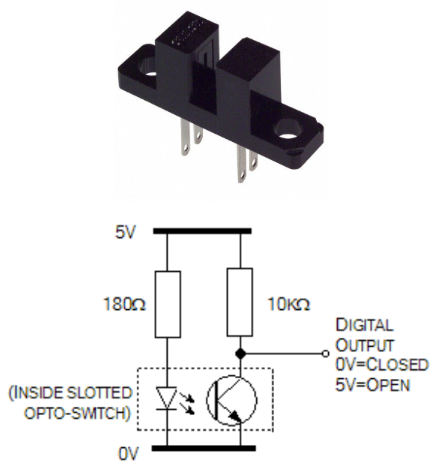
\includegraphics[scale=1]{./images/slotted-opto-switch.png}
\end{center}
\subsection{Data acquisition (DAQ)}
\label{sec:org322be30}
Data acquisition is the process of sensing a physical state and converting it into a digital form for processing, presentation and storage.
\subsection{Digitised signal}
\label{sec:org730aab8}
A digitised signal is a series of numbers which approximates an analogue signal at the sampling time instances. There are two important parameters, sampling rate (x-axis) and digitisation resolution (y-axis).
\subsection{Shannon sampling theorem}
\label{sec:org944b22e}
The Shannon sampling theorem states that there is no maximum sampling frequency, higher sampling frequency also means more noise and higher costs. It also states that the sampling frequency (\(f_s\)) must be at least 2 times higher than the highest frequency component (\(f_{max}\)) in the signal, i.e.
\[f_s > 2f_{max} \Longleftrightarrow T_s < \frac{1}{2} T_{min} \quad \because \ \text{Period } T = \frac{1}{f}\]

The Nyquist frequency refers to this frequency, which is \(2f_{max}\).


Consider the following \(\qty{1}{Hz}\) signals:
\begin{center}
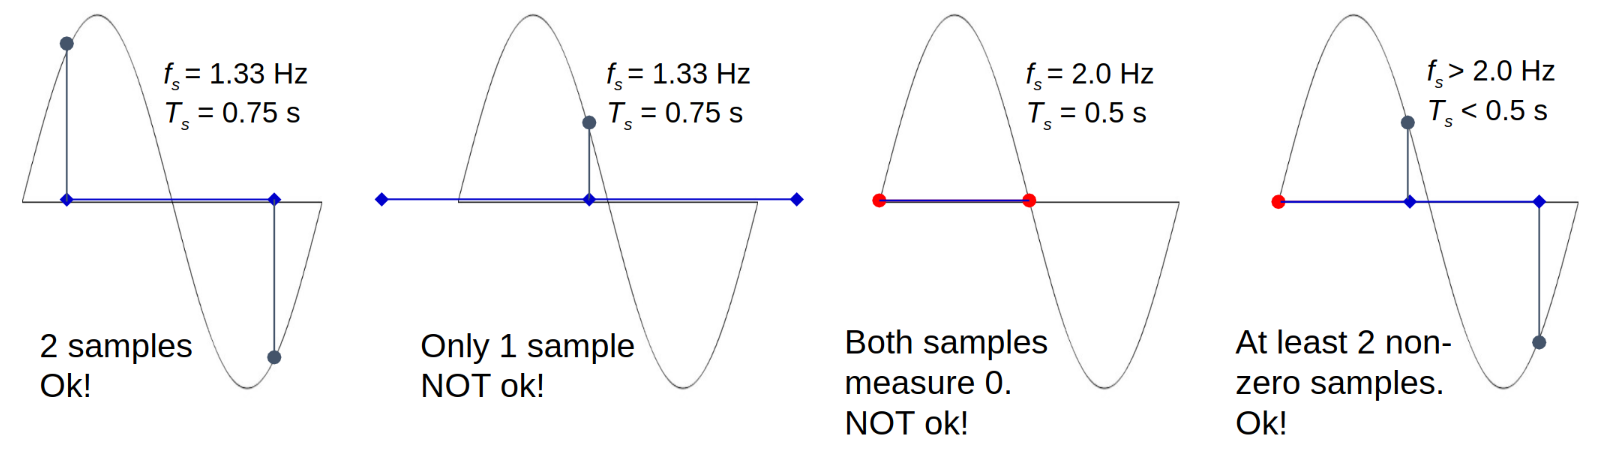
\includegraphics[width=.9\linewidth]{./images/shannon-sampling-theorem.png}
\end{center}

 \newpage
\subsection{Aliasing}
\label{sec:orga502ef6}
Aliasing is an effect that causes different signals to become indistinguishable (or aliases of one another) as a result of undersampling.

Example:
\begin{itemize}
\item The original signal is 10 cycles at \(f_0\).
\item The sampling frequency \(f_s\) is \(1.2 f_0\).
\item There is a total of 12 sampling points.
\item The resulting sampled signal appears to be \(0.2 f_0\).
\end{itemize}

\begin{center}
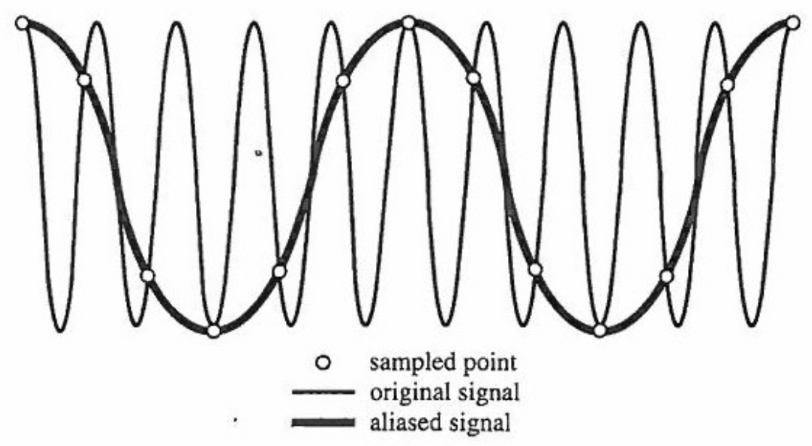
\includegraphics[width=.9\linewidth]{./images/aliasing-example.png}
\end{center}
\subsection{Quantising theory}
\label{sec:org55979b4}
\begin{center}
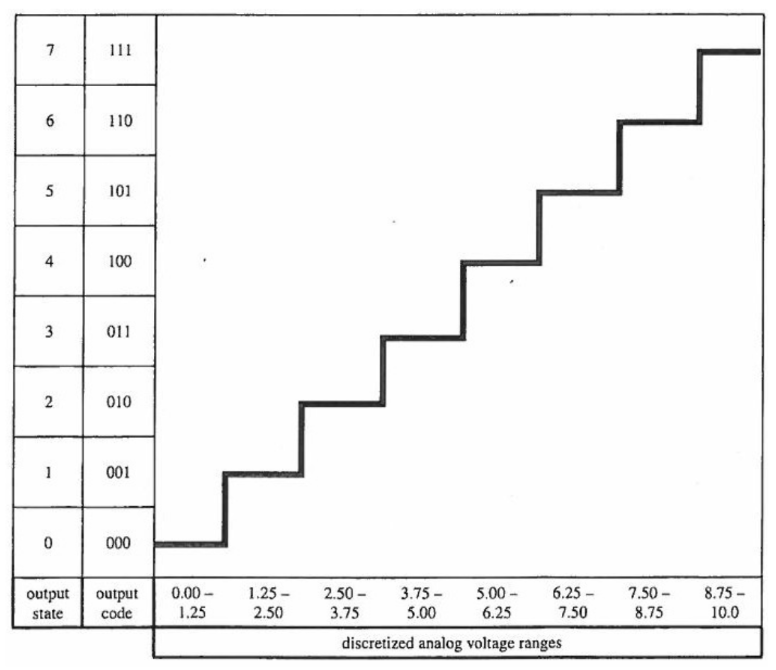
\includegraphics[width=.9\linewidth]{./images/quantising-theory.png}
\end{center}
\subsubsection{Quantising}
\label{sec:orgecf95b4}
Quantising refers to the conversion of a continuous analogue signal to a series of discrete states.
\subsubsection{Coding}
\label{sec:org305d5a4}
Coding refers to the assignment of a digital code number to each state.
\subsubsection{Number of states}
\label{sec:org4da2b48}
The number of states is given by:
\[N = 2^n \text{ for the states } 0 \ldots N - 1\]

Where:
\begin{itemize}
\item \(N\) is the number states
\item \(n\) is the number of bits of the analogue to digital conversion
\end{itemize}
\subsection{Pulse width modulation}
\label{sec:orgcd7805a}
Pulse width modulation varies the duty cycle or the duration of a pulse to control the average power or amplitude delivered by an electrical signal.
\subsubsection{Example}
\label{sec:orga863e5c}
\begin{itemize}
\item If a switch is always on, the lamp receives \(\qty{9}{V}\) and lights up to the rated brightness.
\item If a switch is 50\% on and 50\% off very quickly (1 - \(\qty{200}{kHz}\)), the lamp receives and equivalent of \(\qty{4.5}{V}\), and lights up to only 50\% of the rated brightness.
\end{itemize}
\subsection{Inductive kickback}
\label{sec:orge3d3247}
\begin{center}
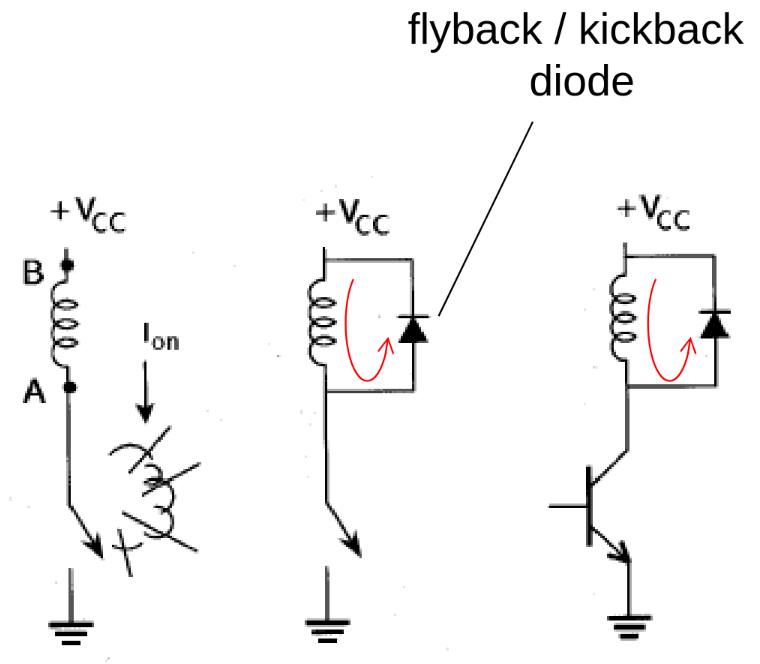
\includegraphics[scale=0.75]{./images/inductive-kickback.png}
\end{center}

\begin{itemize}
\item The steady-state current through an inductor, \(I_{on}\), cannot immediately go to zero when the switch is opened. The changing current induces a voltage across the inductor, making the potential \(A\) greater than \(B\), causing the switch to "blow up".
\item A kickback or flyback diode protects the switch (physical or transistor) from blowing up.
\end{itemize}
\subsection{Servo motor}
\label{sec:orgb4eb6ba}
The drive flange of the servo motor can rotate \(180^{\circ}\). It is driven by width of high pulse (Logic 1) called "Mark" length.

\begin{center}
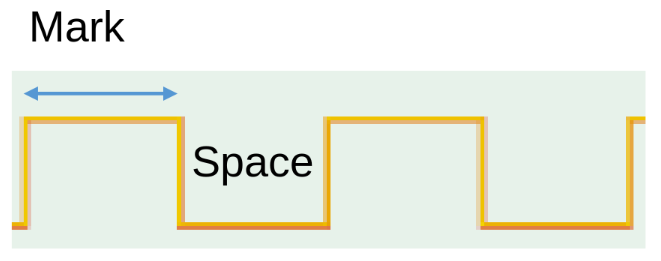
\includegraphics[scale=0.6]{./images/servo-motor-mark-length.png}
\end{center}
\subsubsection{Working principle}
\label{sec:orgac13eeb}
\begin{center}
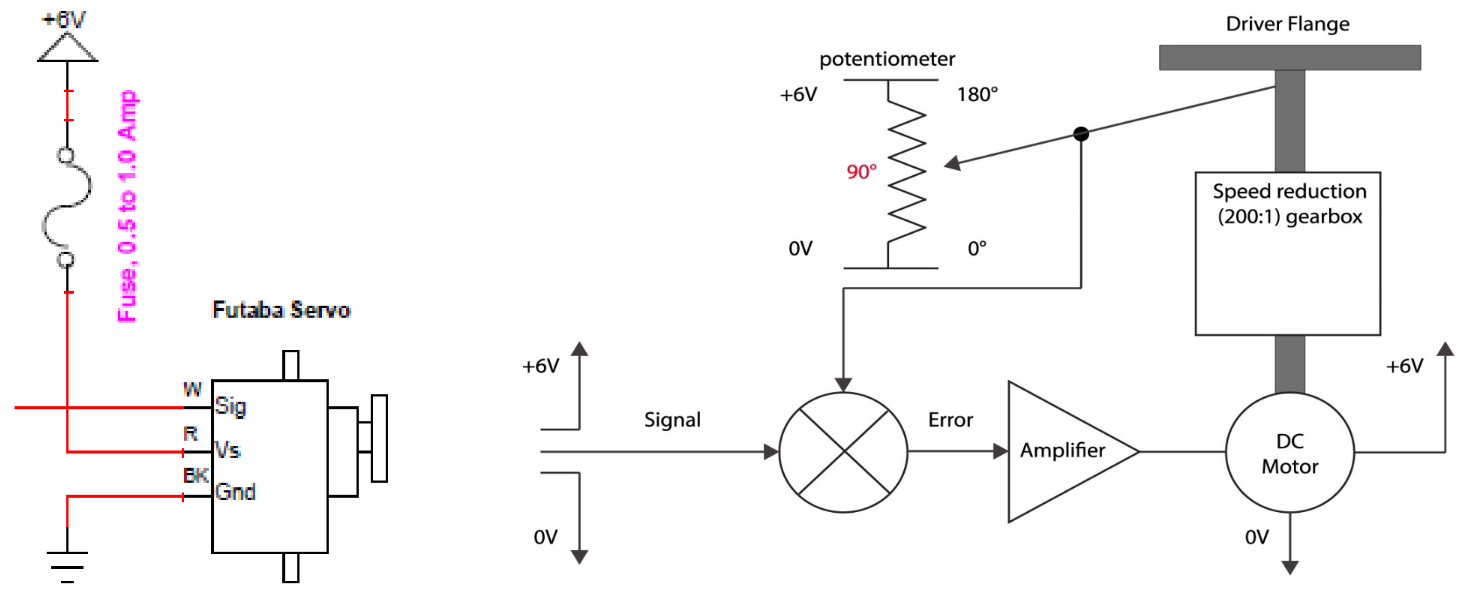
\includegraphics[width=.9\linewidth]{./images/servo-motor-working-principle.png}
\end{center}
\subsubsection{Driving a servo motor}
\label{sec:orgcd8b2d3}
\begin{center}
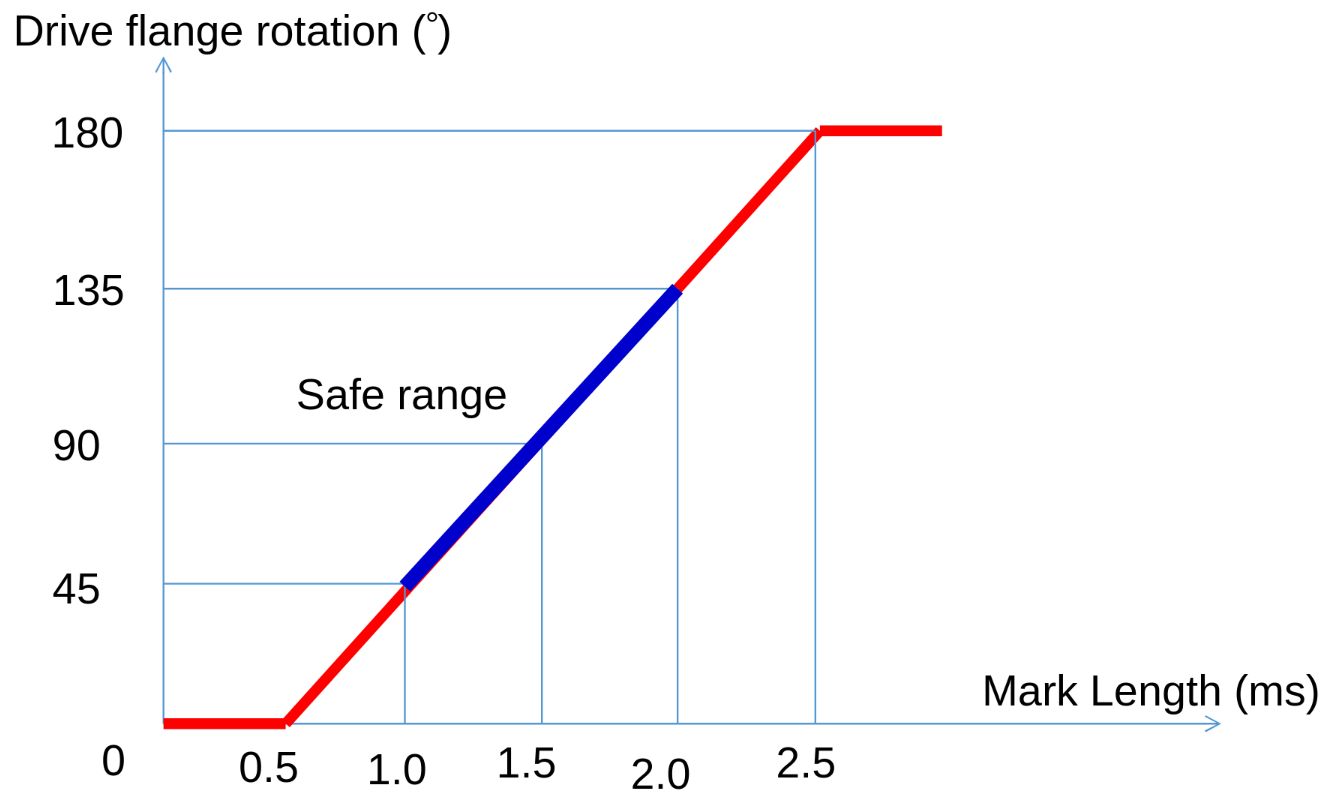
\includegraphics[width=.9\linewidth]{./images/driving-a-servo-motor.png}
\end{center}
\subsection{Stator}
\label{sec:orgd928ee6}
Stator just means an element or part that is static, or doesn't move.
\subsection{Rotor}
\label{sec:org511791b}
Rotor just means an element or part that rotates.
\subsection{Solenoid}
\label{sec:org5f19cdd}
\begin{center}
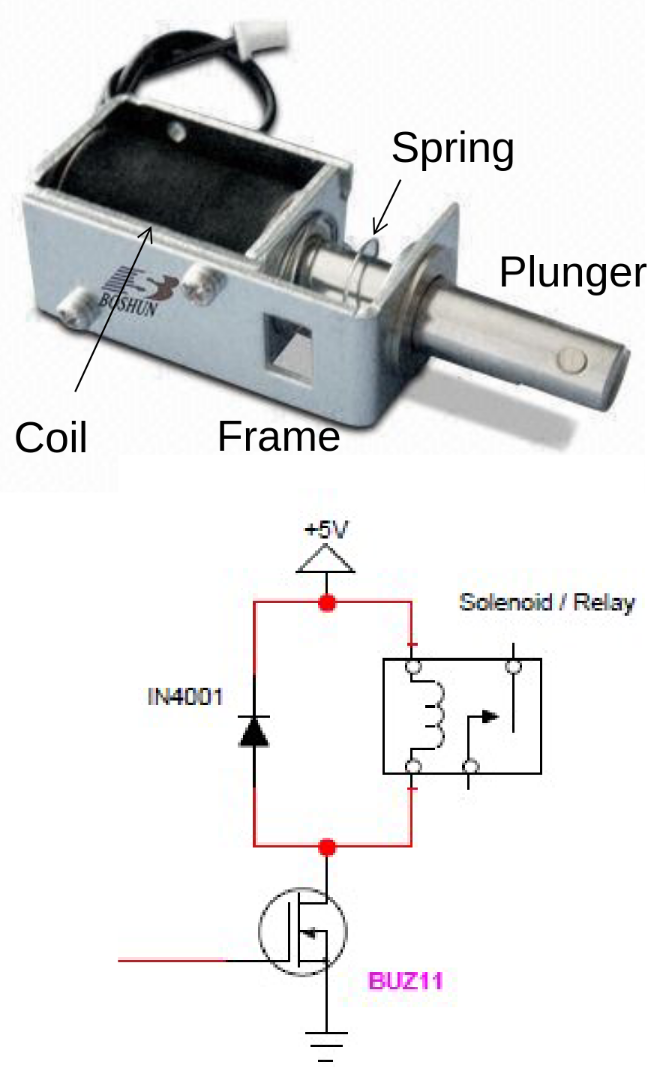
\includegraphics[scale=0.6]{./images/solenoid-diagram.png}
\end{center}
\subsubsection{Construction}
\label{sec:orge93fc22}
\begin{itemize}
\item Stationary iron frame (stator)
\item Coil (solenoid)
\item Ferromagnetic plunger (armature)
\end{itemize}
\subsubsection{Types}
\label{sec:org979fcb3}
A solenoid can be one of two types, a push solenoid or a pull solenoid.
\subsubsection{Control}
\label{sec:org5b84369}
A pulse is used to turn the solenoid on and off.
\subsection{Stepper motor}
\label{sec:orgcf818d4}
\begin{center}
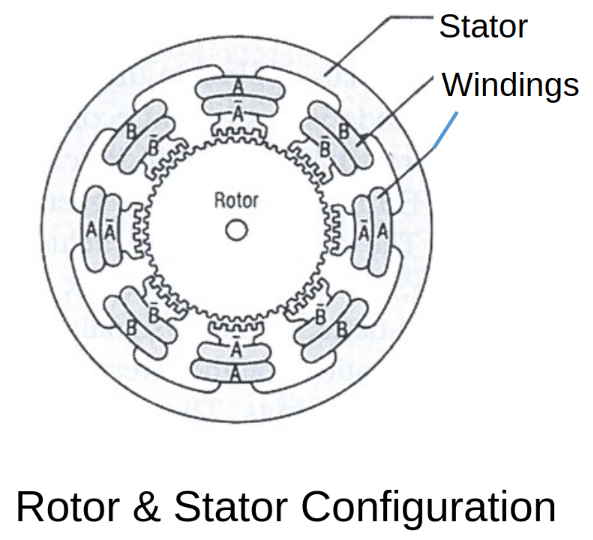
\includegraphics[scale=0.5]{./images/stepper-motor-configuration.png}
\end{center}
\subsubsection{Construction}
\label{sec:org1405cd0}
\begin{center}
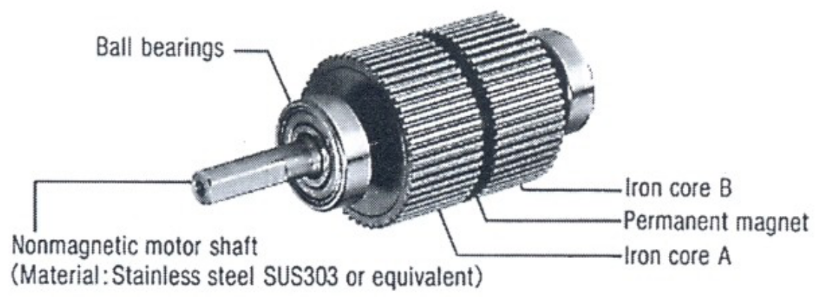
\includegraphics[width=.9\linewidth]{./images/stepper-motor-construction.png}
\end{center}
\begin{itemize}
\item Permanent magnet rotor
\item Stator with rotating magnetic field
\end{itemize}

 \newpage
\subsubsection{Working principle}
\label{sec:org79047b7}
\begin{center}
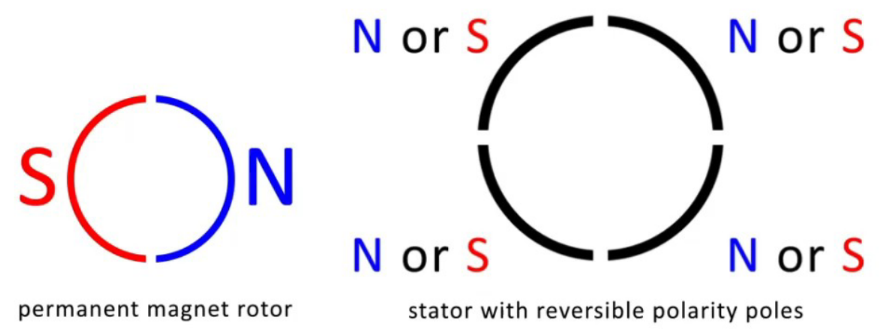
\includegraphics[width=.9\linewidth]{./images/stepper-motor-working-principle-diagram.png}
\end{center}
\begin{itemize}
\item If just one winding of the motor is energized, the rotor will snap (rotate) to a fixed angle and then hold that angle until the torque exceeds the holding torque of the motor.
\item As the polarity of the stator changes, the permanent magnet motor will rotate to the next fixed position.
\item Doubling the number of poles will half the step size, as each step is now smaller.
\end{itemize}
\subsubsection{Wave drive or single phase stepping method}
\label{sec:org5241eb5}
\begin{itemize}
\item In the wave drive or single phase stepping method, only one magnet in the stator is turned on at a time.
\item This means the rotor inside the stepper motor will be attracted to one magnet of the stator of the stepper motor each time it takes a step.
\item The rotor will therefore be aligned to the one magnet each step.
\end{itemize}

 \newpage
\subsubsection{Two phase full step stepping method}
\label{sec:org97d23b5}
\begin{itemize}
\item In the two phase full step stepping method, two magnets beside each other in the stator are turned on at a time.
\item This means the rotor inside the stepper motor will be attracted to both magnets of the stator of the stepper motor each time it takes a step.
\item The rotor will therefore be aligned in between the two magnets of the stator.
\item These two magnets being activated allows the stepper motor to have more holding torque as the magnetic force holding the rotor in place is much higher compared to the wave drive stepper motor.
\item As such, the motor can take a higher payload (more weight can be attached to the stepper motor).
\item However, the motor also consumes more power.
\end{itemize}

 \newpage
\subsubsection{Two phase half step stepping method}
\label{sec:org4ae4bea}
\begin{itemize}
\item In the two phase half step stepping method, the stepper motor alternates between the wave drive stepping method and the two phase full step stepping method.
\item On the first step, the two phase full step stepping method is used, so the rotor will be attracted to two magnets of the stepper motor on the first step, and it will be in between both magnets.
\item On the second step, the wave drive stepping method is used, so the rotor will be attracted to one magnet of the stepper motor on the second step, and it will be aligned to the one activated magnet on the stator.
\item On the third step, the two phase full step stepping method is used, so the rotor will be attracted to two magnets of the stepper motor on the first step, and it will be in between both magnets.
\item On the fourth step, the wave drive stepping method is used, so the rotor will be attracted to one magnet of the stepper motor on the second step, and it will be aligned to the one activated magnet on the stator.
\item This pattern continues for the rest of the steps, with the motor alternating between the two phase full step stepping method and the wave drive stepping method.
\item This stepping method has the advantage of a smaller step resolution than the two phase full step stepping method, as each step of this stepping method is half a step of the two phase full step stepping method.
\end{itemize}

 \newpage
\subsubsection{Micro-stepping}
\label{sec:orga4544a1}
\begin{itemize}
\item Micro-stepping is a way to achieve smaller step resolutions by controlling the fractions of the current flowing into the two magnets being activated in the two phase stepping method individually.
\item This allows the motor to step in fractions of a full step at a time instead of a full step.
\item For example, the second magnet can be powered with one-eighth the current of the first magnet, which will cause the rotor to be much closer to the first magnet than the second magnet, allowing the rotor to rotate one-eighth of a step.
\end{itemize}
\subsection{Handshaking}
\label{sec:orga45f4ca}
Handshaking is the process when the MCU sends a data available (DAV) control signal to an output device, and the output device accepts the data upon receiving the DAV signal, and sends a data accepted (DACK) control signal back to the MCU.

\begin{center}
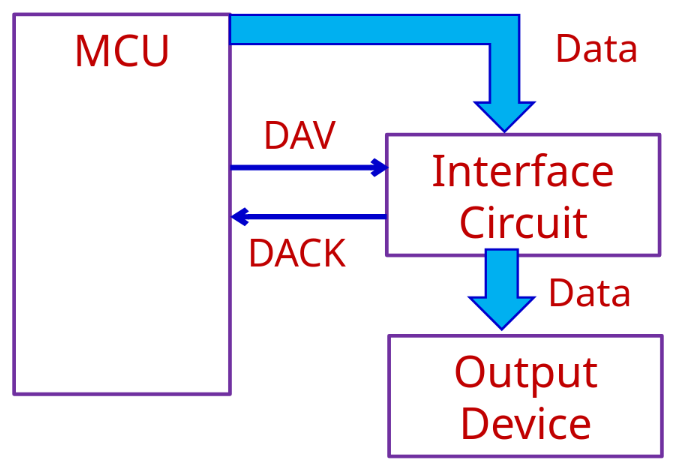
\includegraphics[scale=1]{./images/handshaking-diagram.png}
\end{center}
\subsection{Interrupt service routine (ISR)}
\label{sec:org8f69401}
Interrupt service routine contains the commands for transferring to and from the interrupting I/O devices.

\begin{center}
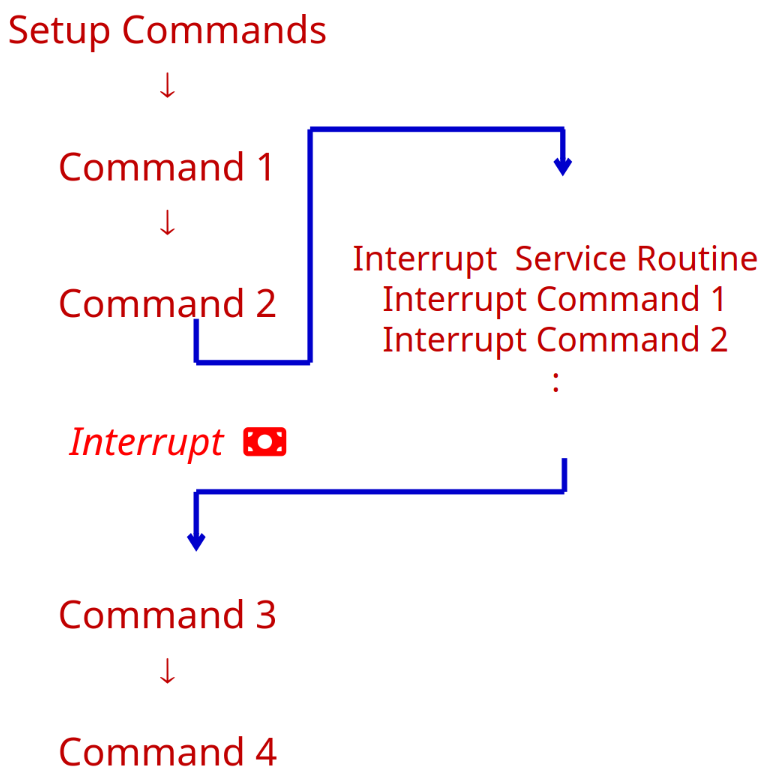
\includegraphics[width=.9\linewidth]{./images/interrupt-service-routine-diagram.png}
\end{center}

 \newpage
\subsubsection{In an Arduino}
\label{sec:orgf4f9b61}
\begin{itemize}
\item The interrupt service routine cannot have parameters and returns nothing.
\item Only 1 interrupt service routine can run at any one time, other interrupt service routines (if any) will be turned off until the current one is executed.
\item Functions which rely on timer interrupts will not work while an interrupt service routine is running, like \texttt{delay()} and \texttt{millis()}.
\item Global variables are used to pass parameters between the main program and the interrupt service routine, so declare these variables as \texttt{volatile}.
\end{itemize}

Example:
\begin{minted}[]{cpp}
int pin = 1;
volatile int state = LOW;

void setup() {
    pinMode(pin, OUTPUT);
    attachInterrupt(0, blink, CHANGE);
}

void loop() {
    digitalWrite(pin, state);
}

void blink() {
    state = !state;
}
\end{minted}
\subsection{Parallel data communications}
\label{sec:orgc173350}
\begin{itemize}
\item Multiple bits of data are transmitted all at one time.
\item One data line or pin per bit is needed.
\item The advantage of parallel data communications is faster data transfer rate.
\end{itemize}
\subsection{Serial data communications}
\label{sec:org7b237cb}
\begin{itemize}
\item Data is transmitted one bit after another
\item Only one data line or pin is needed
\item Advantages:
\begin{itemize}
\item Cheaper to implement as physical pins and data lines are costly.
\item Easier to integrate into IC \& PCB design as fewer physical pins and lines result in a smaller footprint.
\end{itemize}
\end{itemize}
\subsection{Parallel-serial interface}
\label{sec:org5213cf5}
A parallel-serial interface is for serial or parallel conversions for communications between the MPU and a serial I/O device.
\begin{itemize}
\item It converts an N bit parallel word from the MPU data bus to a serial data word.
\item It also converts a serial data signal from a serial device to an N bit parallel data word.
\end{itemize}
\subsection{Bit time interval (\(T_B\))}
\label{sec:org03a74bd}
The bit time interval is the period of time between one bit to another, when transferring data.
\subsection{Baud rate}
\label{sec:org8522c51}
Baud rate is the data rate, or the rate of data transmission, which is measured in bits per second or \(\unit{Mbps}\).

\[\text{Baud rate} = \frac{1}{T_B}\]

Common baud rates are 19200, 14400, 9600, etc.
\subsubsection{Example}
\label{sec:orge5c677a}
If the data rate (baud rate) is 9600 baud, what is the time duration of 1 bit?
\begin{itemize}
\item The data rate is 9600 bits per second
\item The bit time is \(\frac{1}{9600} = \qty{104.17}{\micro s}\)
\end{itemize}
\subsection{Universal asynchronous receiver and transmitter (UART)}
\label{sec:org0f5104c}
\begin{itemize}
\item It uses one to one communication, which means a pin receives the data and another pin transmits the data.
\item For the Arduino Uno, digital pin 0 is the Rx pin and digital pin 1 is the Tx pin.
\item For other pins that don't have hardware serial, use the \texttt{SoftwareSerial} library to use them for communication.
\item It consists of the following components:
\end{itemize}
\subsubsection{Serial receiver (Rx)}
\label{sec:org94b1089}
A serial receiver converts a serial input to a parallel format, and stores it in the receiver data register (RxDR) for eventual transmission to the MPU. For the Arduino Uno, this is digital pin 0.
\subsubsection{Serial transmitter (Tx)}
\label{sec:org8028467}
A serial transmitter takes a parallel word from the transmitter data register (TxDR) and converts it to a serial format for transmission. For the Arduino Uno, this is digital pin 1.
\subsubsection{Bidirectional data bus buffer}
\label{sec:org2ea7e4b}
A bidirectional data bus buffer is to pass data from the MPU to the transmitter data register (TxDR) or from the receiver data register (RxDR) to the MPU over the system bus.
\subsubsection{Baud rate generator}
\label{sec:org81d4313}
Sometimes an external clock is used instead of the timer on the Arduino.
\subsubsection{How UART works}
\label{sec:orga1c4f46}
\begin{center}
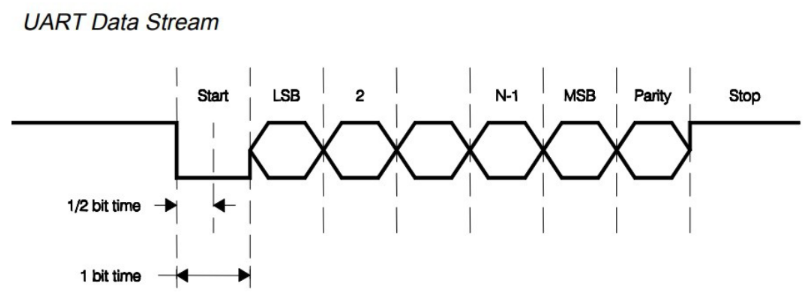
\includegraphics[width=.9\linewidth]{./images/uart-data-stream-diagram.png}
\end{center}
\begin{enumerate}
\item It first organises data into packets, and each packet contains:
\begin{itemize}
\item 1 start bit (LOW)
\item 5 - 9 data bits
\item 1 optional parity bit, to validate that the data is transferred correctly
\item 1 - 2 stop bits (HIGH)
\end{itemize}
\item Read the data according to the baud rate.
\end{enumerate}
\subsection{Bus}
\label{sec:org7d35eba}
A bus is a group of wires used as a common path connecting all the inputs and outputs of several registers and devices so that the data can be easily transferred from any one register or device to any other using various control signals.
\subsection{Asynchronous communication}
\label{sec:org7546a24}
\begin{itemize}
\item The transmitter can send data to the receiver at any time.
\item The time delay between the transmission of two words may be indeterminate.
\item Transmitter clock need not synchronise with the receiver clock.
\end{itemize}

 \newpage
\subsection{Synchronous communication}
\label{sec:orged7e152}
\begin{itemize}
\item Transmitting and receiving are synchronised by common clock pulses.
\item Transmitter sends data to receiver continually.
\item Transmitter sends meaningless data, like the ASCII sync character 16\textsubscript{16} continually when there is no data to send.
\end{itemize}
\subsection{Inter-integrated Circuit (I2C) Bus}
\label{sec:org7e70a81}
\begin{itemize}
\item I2C bus is controlled by a master device, which is usually the MCU.
\item One or more slave devices, usually an I/O device, receives the control signal from the master device.
\item All devices share the same clock signal (SCL) and a bidirectional data line (SDA), and hence there are only 2 signal lines.
\item Only the master device can initiate communications between master and slaves to avoid bus contention.
\item Each slave device has its own unique 7-bit address or ID number. This address may be fixed or selectable, and is dependent on the manufacturer.
\item Each signal line requires a pull-up resistor to restore the signal to HIGH when no device is set to LOW.
\item When a master device initiates a communication, a device address is transmitted.
\item Only the slave device with the correct address shall respond to the master.
\end{itemize}

\begin{center}
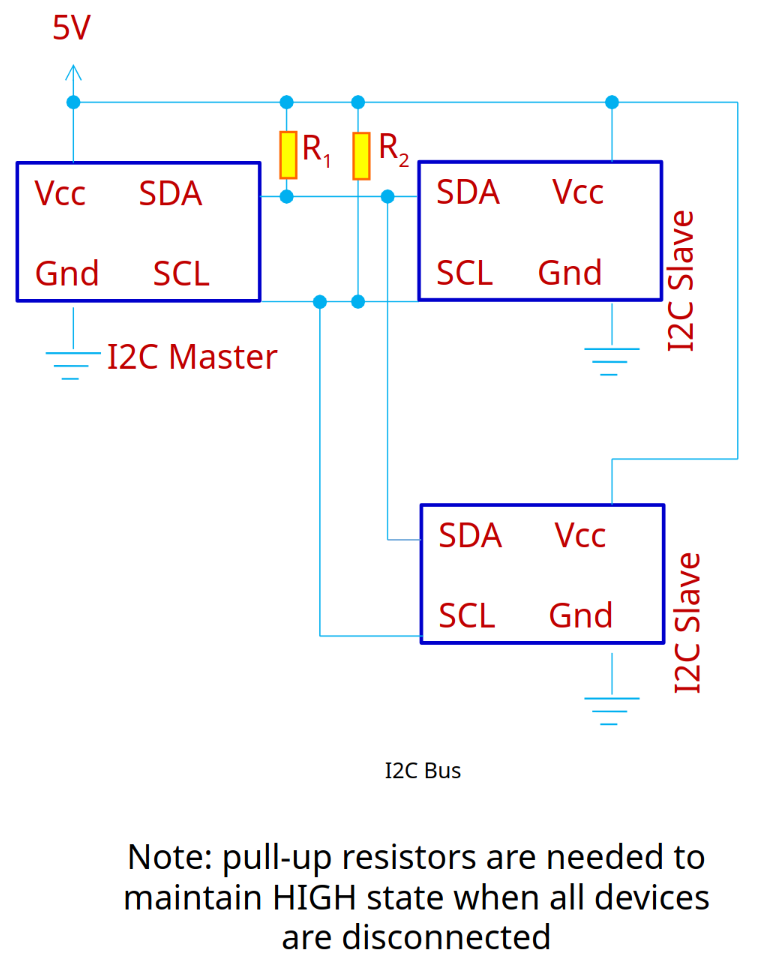
\includegraphics[scale=0.6]{./images/i2c-bus-diagram.png}
\end{center}
\subsubsection{Communication protocol}
\label{sec:org6d23aca}
Steps to communicate with different I2C slave devices need to follow protocol defined by manufacturers in the provided data sheets.


Basic steps:
\begin{enumerate}
\item Master sends a Start bit.
\item Master sends a 7-bit slave address of intended device.
\item Master sends a Read (1) or Write (0) bit depending on application.
\item Slaves responds with an "acknowledge", i.e. ACK bit (0).
\item In Write mode, master sends 1 byte of information (command or data) at a time, and slaves respond with ACKs. In Read mode, master receives 1 byte of information at a time and sends an ACK to the slave after each byte.
\item When communication has been completed, master sends a Stop bit.
\end{enumerate}
\subsubsection{On the Arduino}
\label{sec:org381eb5e}
\begin{itemize}
\item Use the \texttt{Wire.h} library to use I2C communication.
\item Analogue pin A4 is the bidirectional data line (SDA).
\item Analogue pin A5 is the line for the same clock signal (SCL).
\item The data is transferred in 8 bits.
\item To read data, a request for data must be sent first using \texttt{Wire.requestFrom(address, quantity, stop)}.
\begin{itemize}
\item Address refers to the 7-bit address of the device to request data from.
\item Quantity refers to the number of bytes to request.
\item Stop is a boolean. When set to \texttt{true}, the protocol will send a stop message after the request, releasing the bus. When set to \texttt{false}, it will continually send a repeated start message after the request, keeping the connection active.
\end{itemize}
\end{itemize}
\subsubsection{I2C vs SPI}
\label{sec:org06d5ed2}
\begin{center}
\begin{tabular}{l|l}
I2C advantages & SPI advantages\\
\hline
Requires only 2 communication lines & Higher data transmission rate\\
 & Easier to implement\\
 & No pull-up resistors needed\\
\end{tabular}
\end{center}
\subsection{Full-duplex}
\label{sec:org1a6d199}
Full-duplex means simultaneous bidirectional transmission of information.

 \newpage
\subsection{Serial Peripheral Interface (SPI) bus}
\label{sec:orgfd1107f}
SPI bus is a full-duplex serial communication protocol between master and one or more slaves. It is an interface bus used to send data between microcontrollers and small peripherals such as shift registers, sensors, and SD cards.

\begin{itemize}
\item There are 3 pins for communications between master and all slaves
\begin{itemize}
\item Shared or Serial Clock (SCLK)
\item Master Out Slave In (MOSI) or Slave Data In (SDI)
\item Master In Slave Out (MISO) or Slave Data Out (SDO)
\end{itemize}
\item Each slave device requires an additional slave select (SS) or chip select (CS) pin, so 1 slave select (SS) or chip select (CS) line is needed for each slave device.
\begin{itemize}
\item This line is normally held HIGH to disconnect the slave.
\item When it is brought to LOW, communication is initiated with the slave.
\item It is brought to HIGH again after communication has completed.
\end{itemize}
\item The total number of I/O pins required is \(3 + n\), where \(n\) is the number of slave devices.
\item All slave devices share MOSI, MISO and SCLK lines, hence all commands from the master are sent to each slave device.
\item Every clock cycle a bit must be sent and received (i.e. synchronous), but that bit may be meaningless.
\end{itemize}

\begin{center}
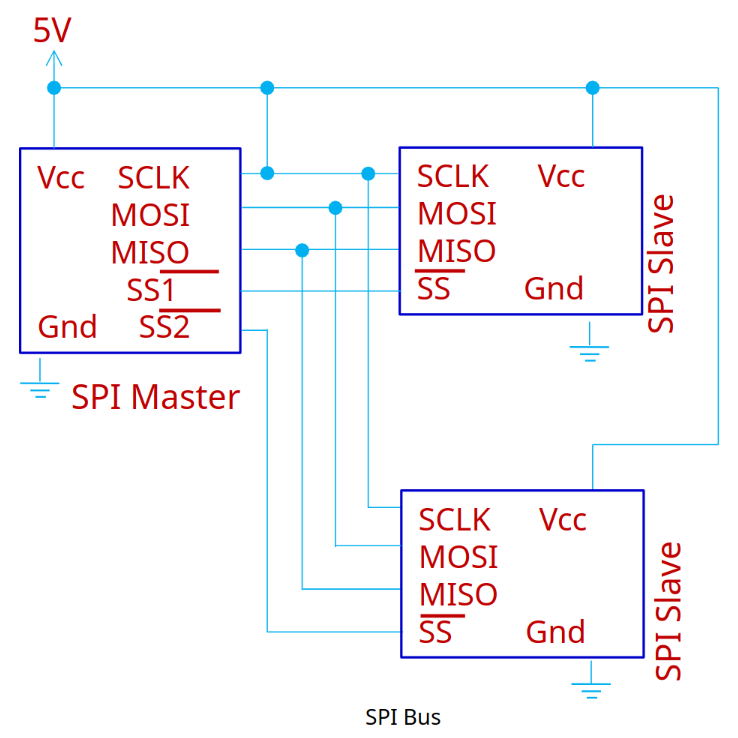
\includegraphics[width=.9\linewidth]{./images/spi-bus-diagram.png}
\end{center}
\subsubsection{Modes of communication}
\label{sec:org301118d}
SPI devices are synchronous, i.e. data is transmitted in sync with a SCLK. There are 4 modes of communication.

\begin{center}
\begin{tabular}{m{2.5em}|m{10em}|m{15em}}
Mode & Clock polarity & Clock phase (data capture on \ldots{})\\
\hline
0 & Low at idle & Rising edge\\
1 & Low at idle & Falling edge\\
2 & High at idle & Falling edge\\
3 & High at idle & Rising edge\\
\end{tabular}
\end{center}

 \newpage
\subsubsection{Communication protocol}
\label{sec:org9c48144}
Basic process:
\begin{enumerate}
\item Set the SS pin to LOW for the targeted slave device
\item Toggle SCLK (square wave) at a speed that is less than or equal to the transmission speed supported by the slave device.
\item For each clock cycle, master sends 1 bit on MOSI and receives 1 bit on MISO.
\item Continue until data transmission is complete, and stop toggling the clock line.
\item Set SS pin to HIGH.
\end{enumerate}
\subsubsection{On the Arduino Uno}
\label{sec:org25fa67a}
\begin{itemize}
\item Use the \texttt{SPI.h} library to use SPI communication.
\item Digital pin 11 is the MOSI pin.
\item Digital pin 12 is the MISO pin.
\item Digital pin 13 is the SCK pin.
\item Digital pin 10 is the SS pin.
\item \texttt{SPISettings(speed, MSB/LSB, mode)}
\begin{itemize}
\item Speed is the rated data transfer speed of the slave in bits per second.
\item Most Significant Bit (MSB) or Least Significant Bit (LSB) first.
\item Mode:
\begin{center}
\begin{tabular}{llll}
Mode & Clock Polarity (CPOL) & Output Edge & Data Capture\\
\hline
\texttt{SPI\_MODE0} & Low at idle & Falling & Rising\\
\texttt{SPI\_MODE1} & Low at idle & Rising & Falling\\
\texttt{SPI\_MODE2} & High at idle & Rising & Falling\\
\texttt{SPI\_MODE3} & High at idle & Falling & Rising\\
\end{tabular}
\end{center}
\end{itemize}
\end{itemize}
\subsubsection{Communication using SPI in the Arduino}
\label{sec:org9b32e51}
\begin{itemize}
\item The slave select or chip select pin must be set to LOW to enable communication first, i.e. \texttt{digitalWrite(10, LOW)}
\item SPI transfer works in two steps, and the first step is to send a byte to the slave device.
\item The first bit of this byte (8 bits) is the read or write bit. Set this bit to 1 to read, and 0 to write.
\item The second bit is the multiple byte (MB) bit, which when set to 1, allows the SPI communication protocol to transfer multiple bytes at once, instead o just one byte at a time. The next byte transferred from the slave device is the register address that is 1 more than the current register address.
\item When this second bit is set to 0, the SPI communication must be terminated, i.e. slave select or chip select pin set to HIGH, \texttt{digitalWrite(10, HIGH)}, after the data is read or written.
\item The third bit to the eighth bit holds the register address to read or write from, which is determined from the data sheet of the slave device.
\item The second step is to read or write the data.
\item For a read operation, transfer a 0 to the slave device, i.e. \texttt{SPI.transfer(0)}.
\item For a write operation, send a byte that corresponds to the operation to perform on the address sent in the first step, which can be obtained from the slave device's data sheet.
\end{itemize}
\subsubsection{I2C vs SPI}
\label{sec:org26bf72a}
\begin{center}
\begin{tabular}{l|l}
I2C advantages & SPI advantages\\
\hline
Requires only 2 communication lines & Higher data transmission rate\\
 & Easier to implement\\
 & No pull-up resistors needed\\
\end{tabular}
\end{center}
\subsection{16-key hexadecimal keypad}
\label{sec:org2595c34}
\begin{center}
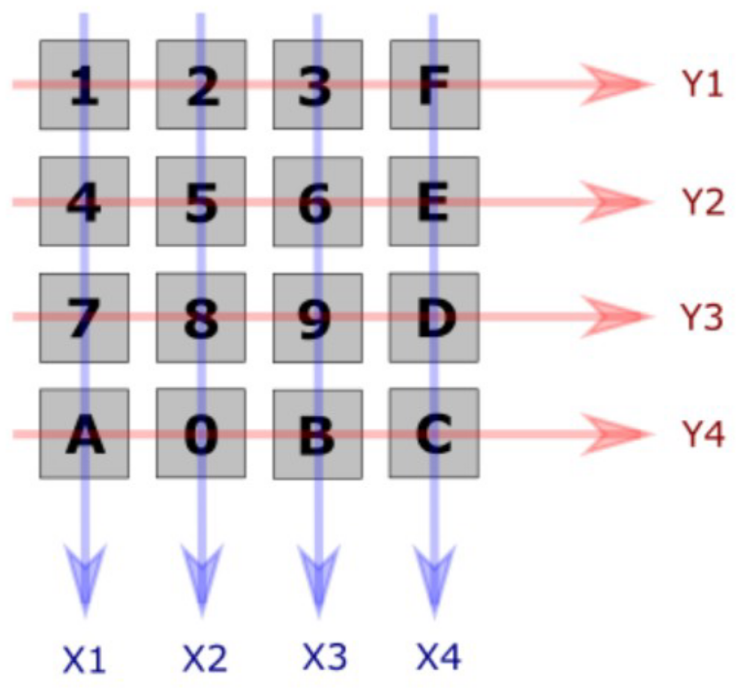
\includegraphics[width=.9\linewidth]{./images/16-key-hexadecimal-keypad.png}
\end{center}
The 16-key hexadecimal keypad has 8 outputs, and hence requires 8 pins.
\subsection{74C922 keypad encoder}
\label{sec:org75805cc}
\begin{center}
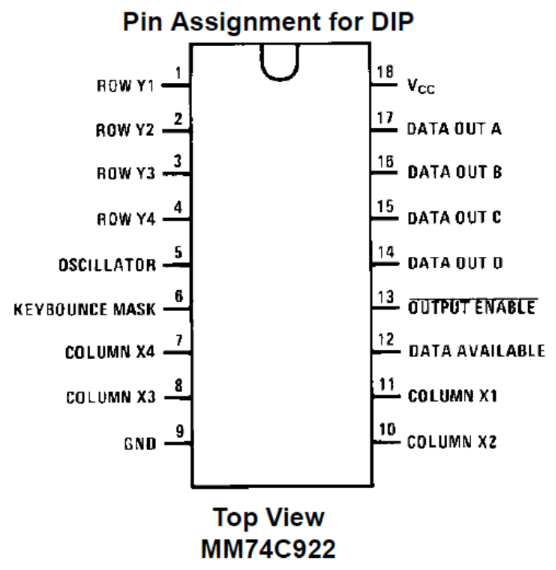
\includegraphics[width=.9\linewidth]{./images/74c922-keypad-encoder.png}
\end{center}
The 74C922 keypad encoder has 8 inputs for the keypad and 4 outputs to the Arduino. The data available pin tells the Arduino that the keypad has been pressed.
\subsubsection{Position of the key pressed}
\label{sec:org69e2d61}
\begin{center}
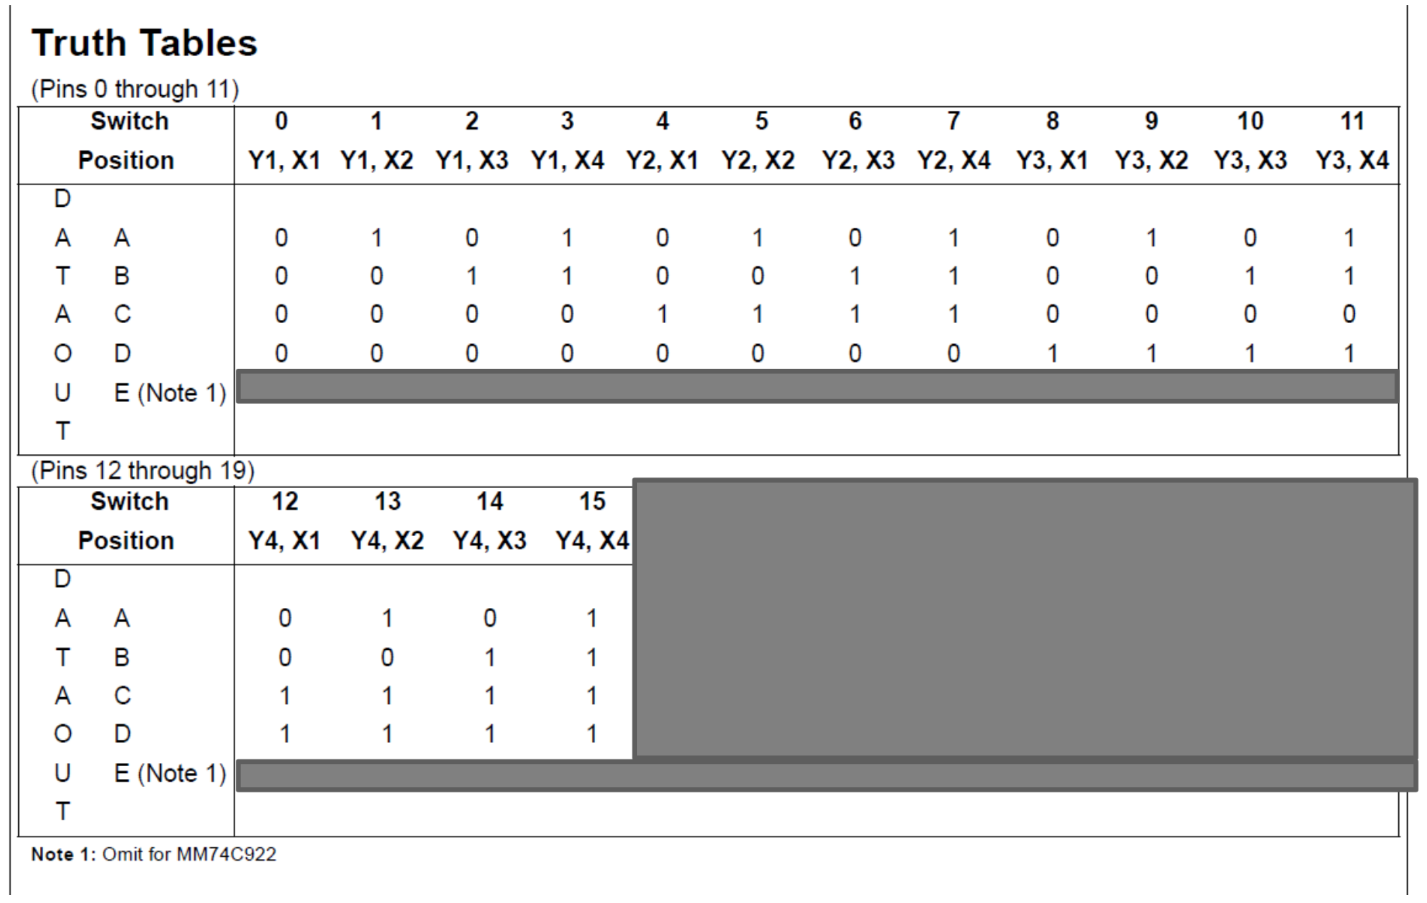
\includegraphics[width=.9\linewidth]{./images/74c922-keypad-encoder-truth-table.png}
\end{center}
\[\text{Position} = A + 2 \cdot B + 4 \cdot C + 8 \cdot D\]

 \newpage
\subsection{Input signal conditioning}
\label{sec:org81135e9}
Input signal conditioning is to convert the output of sensing elements into a form suitable for further processing.
\subsubsection{Types}
\label{sec:orgbcd3a27}
\begin{itemize}
\item Analogue-to-Digital conversion
\item Reducing noise level
\item Enhancing a signal's power
\item Improving noise immunisation
\item Eliminate non-linearity
\end{itemize}
\subsection{Output signal conditioning}
\label{sec:org1f303bc}
Output signal conditioning is to convert the output of digital control systems, like the MCU or the PC, into a form suitable for interfacing with output elements.
\subsubsection{Types}
\label{sec:org025fbf7}
\begin{itemize}
\item Digital-to-Analogue conversion
\item Amplifying signals
\item Improving noise immunisation
\end{itemize}
\subsection{Noise}
\label{sec:orga5f5db1}
\begin{itemize}
\item Noise is unwanted signal.
\item White noise is a signal with equal power in all frequencies and zero mean, i.e. a totally random signal.
\item Coloured noise is unwanted signal with certain bias or distinctive frequencies. An example of coloured noise is leaves falling from a tree when the wind is blowing. The mean of the leaves spread is no longer at the foot of the tree, i.e. the mean or bias is non-zero.
\end{itemize}
\subsection{Signal-to-noise ratio}
\label{sec:org045c8c2}
\begin{itemize}
\item Signal-to-noise ratio is defined as the ratio of the power of a signal (meaningful information) and the power of the background noise (unwanted signal).
\[SNR = \frac{\text{Total signal power}}{\text{Total noise power}} = \frac{w_S}{w_N}\]
\item Expressed in decibels:
\[SNR = 10 \log_{10} \left(\frac{w_S}{w_N} \right) \unit{dB}\]
\end{itemize}
\subsection{Arcing}
\label{sec:org565ef3b}
Arcing is the process of raising the potential to cause electrical current to flow between the anode and cathode through the inert gases inside the tube of a fluorescent light.
\subsection{Logic level converter}
\label{sec:org73a7ad5}
A logic level converter converts from \(\qty{5}{V}\) to \(\qty{3.3}{V}\).
\subsection{Bitwise OR}
\label{sec:org1895efc}
Bitwise OR returns 0 only if both inputs are 0, otherwise it returns a 1. Using bitwise OR with 0 is the identity operation for binary, like how multiplication by 1 just gives you back the same number, the bitwise OR operation with 0 returns the same bit back.

 \newpage
\section{Mechatronics system components}
\label{sec:orgfcdc3e8}
\begin{center}
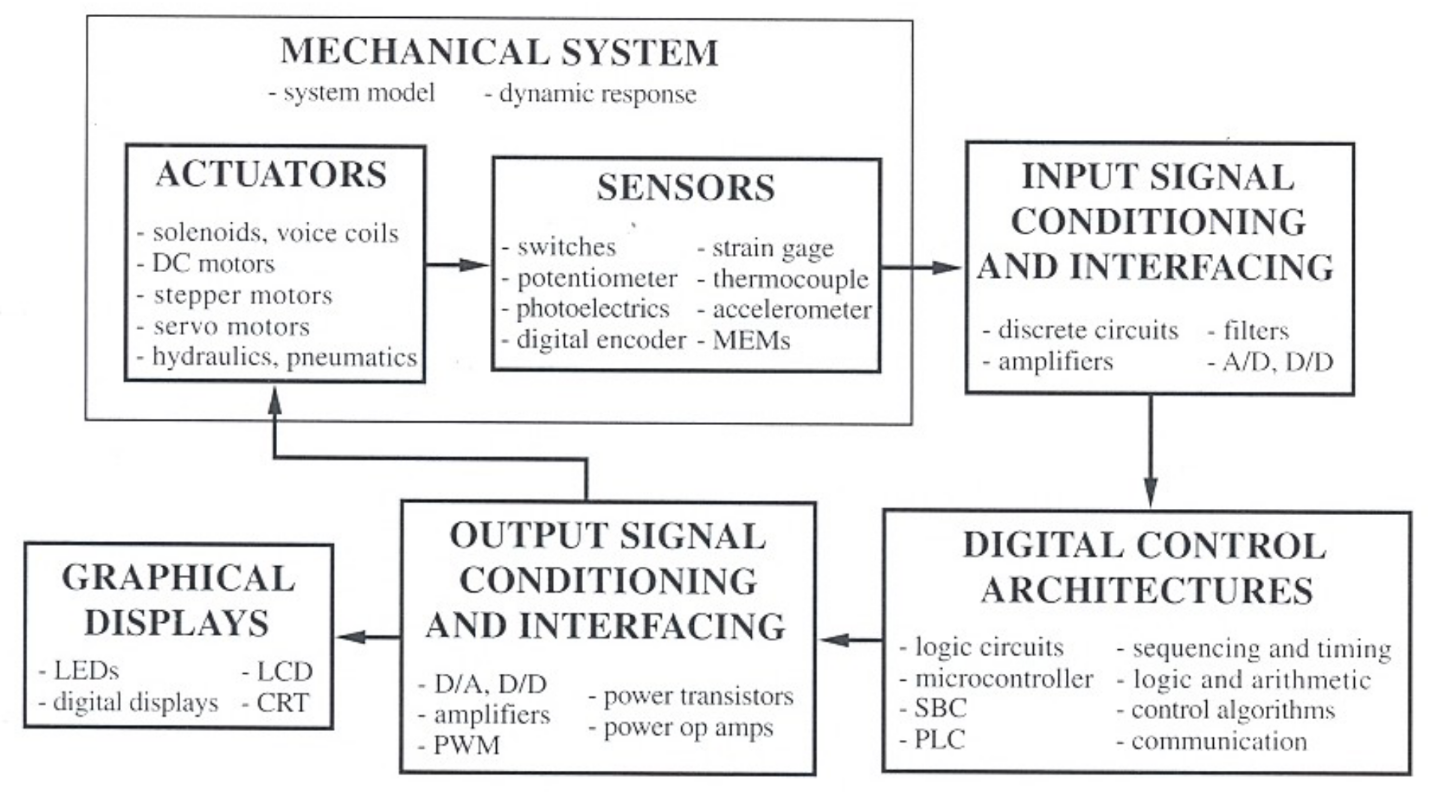
\includegraphics[width=.9\linewidth]{./images/mechatronics-system-components-overview.png}
\end{center}
\subsection{Mechanical system}
\label{sec:org59d2deb}
A mechanical system is when you put the actuators and sensors together.
\subsubsection{Actuators}
\label{sec:org09a5406}
\begin{itemize}
\item Motors (AC motors, DC motors, Stepper motors, Servo motors, Voice coil, etc.)
\item Hydraulics, pneumatics, solenoids
\item Piezoelectrics and other smart materials
\item Others elements like heating and cooling elements
\end{itemize}

 \newpage
\subsubsection{Sensors}
\label{sec:org68168a4}
\begin{itemize}
\item Switches for turning things on and off
\item Potentiometer and encoder for position or displacement
\item Inertial sensors:
\begin{itemize}
\item Accelerometer for acceleration
\item Rate gyroscope for angular velocity
\end{itemize}
\item Thermocouple for temperature
\item Strain Gage for deflection
\item Photoelectrics for light intensity
\end{itemize}

 \newpage
\subsubsection{System model}
\label{sec:org8021c71}
\begin{itemize}
\item First order system, which consists of a damper and a spring.
\begin{center}
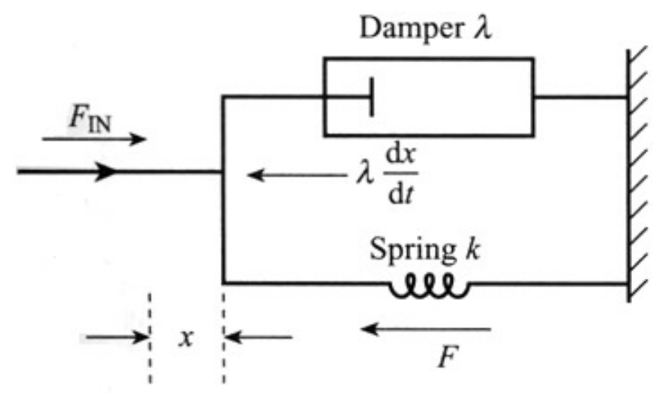
\includegraphics[width=.9\linewidth]{./images/first-order-system-diagram.png}
\end{center}
\[F_{in} - F = \lambda \frac{dx}{dt}\]

\item Second order system, which also consists of a damper and a spring, but the mass is no longer negligible.
\begin{center}
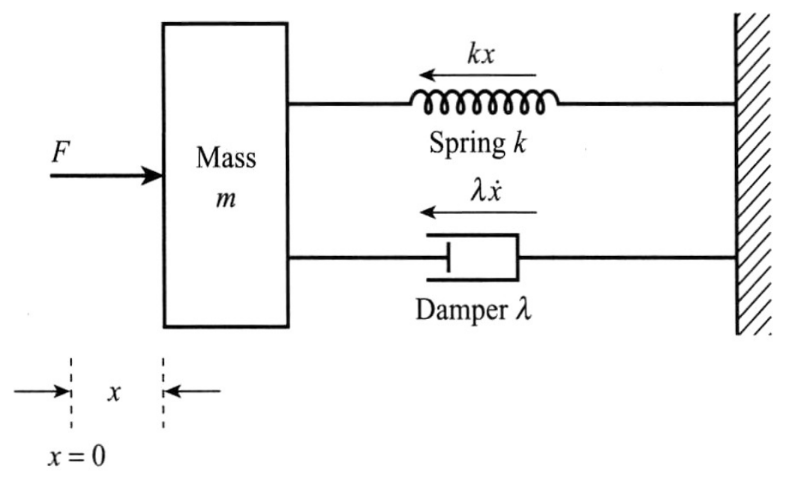
\includegraphics[width=.9\linewidth]{./images/second-order-system-diagram.png}
\end{center}
\[m \ddot{x} + \lambda \dot{x} + kx = F\]
\end{itemize}
\subsubsection{Static and dynamic responses}
\label{sec:orgfb9a5f6}
\begin{itemize}
\item Step response
A step response is like dropping an accelerometer to induce a sudden acceleration. This step response is essentially the input into the mechanical system.

\begin{center}
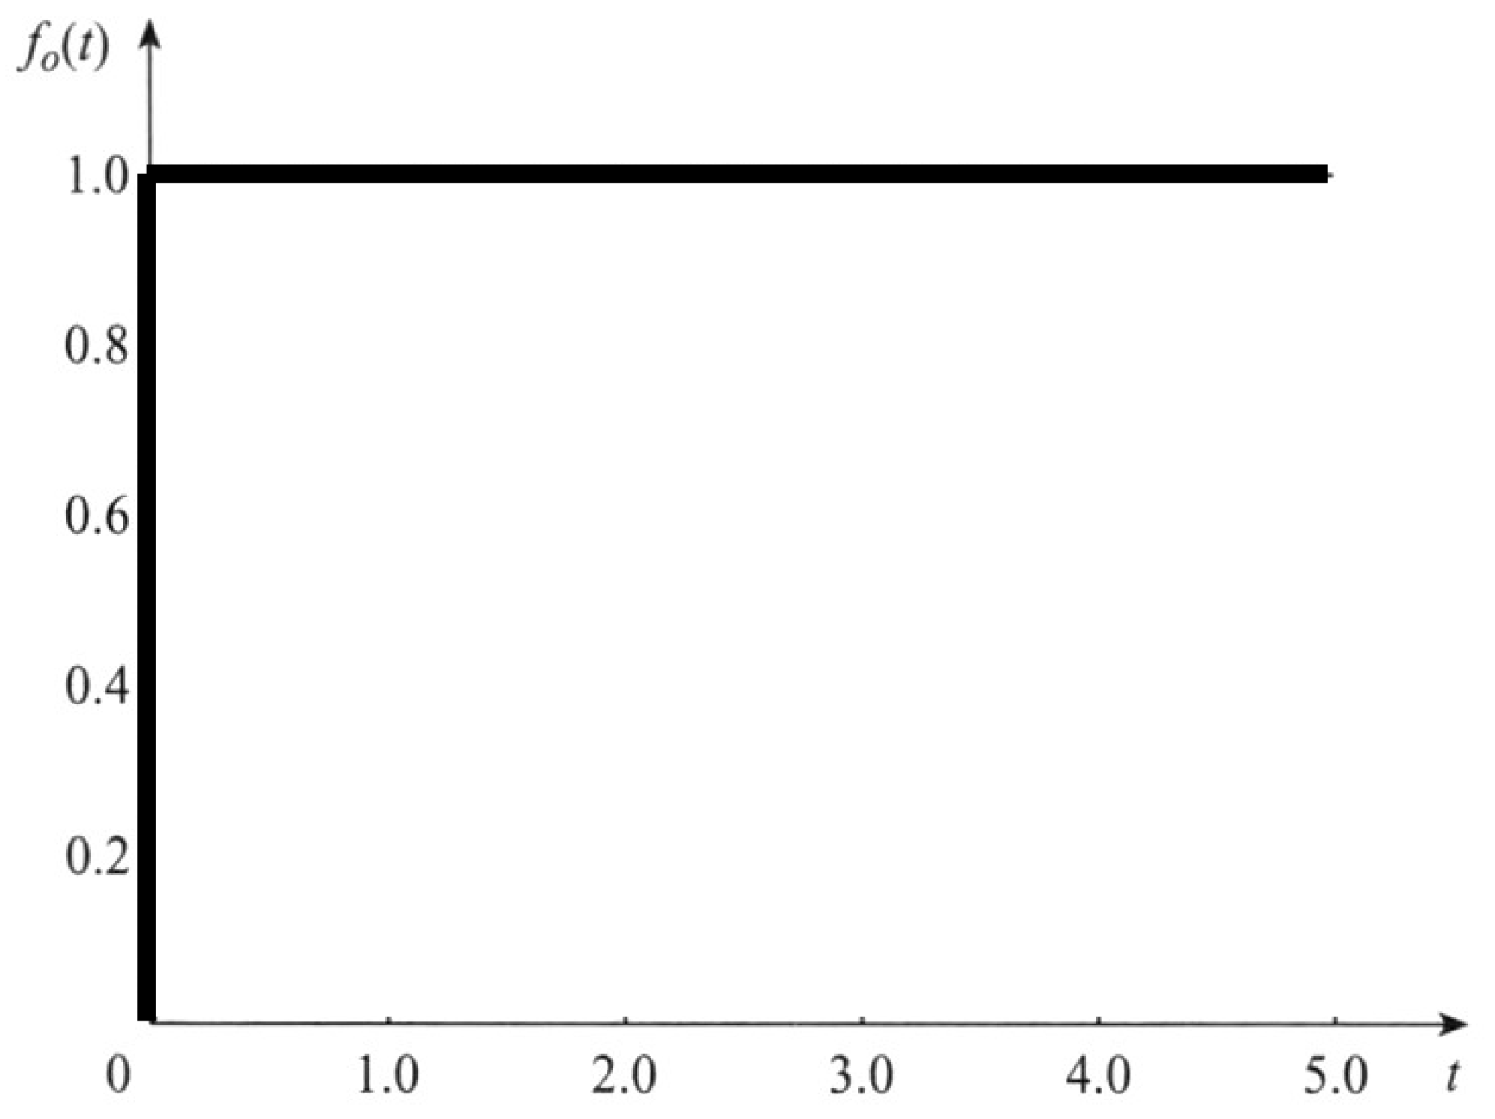
\includegraphics[scale=0.4]{./images/step-response.png}
\end{center}

\item 1st order
A 1\textsuperscript{st} order system will behave in response to a step response as shown in the graph below:

\begin{center}
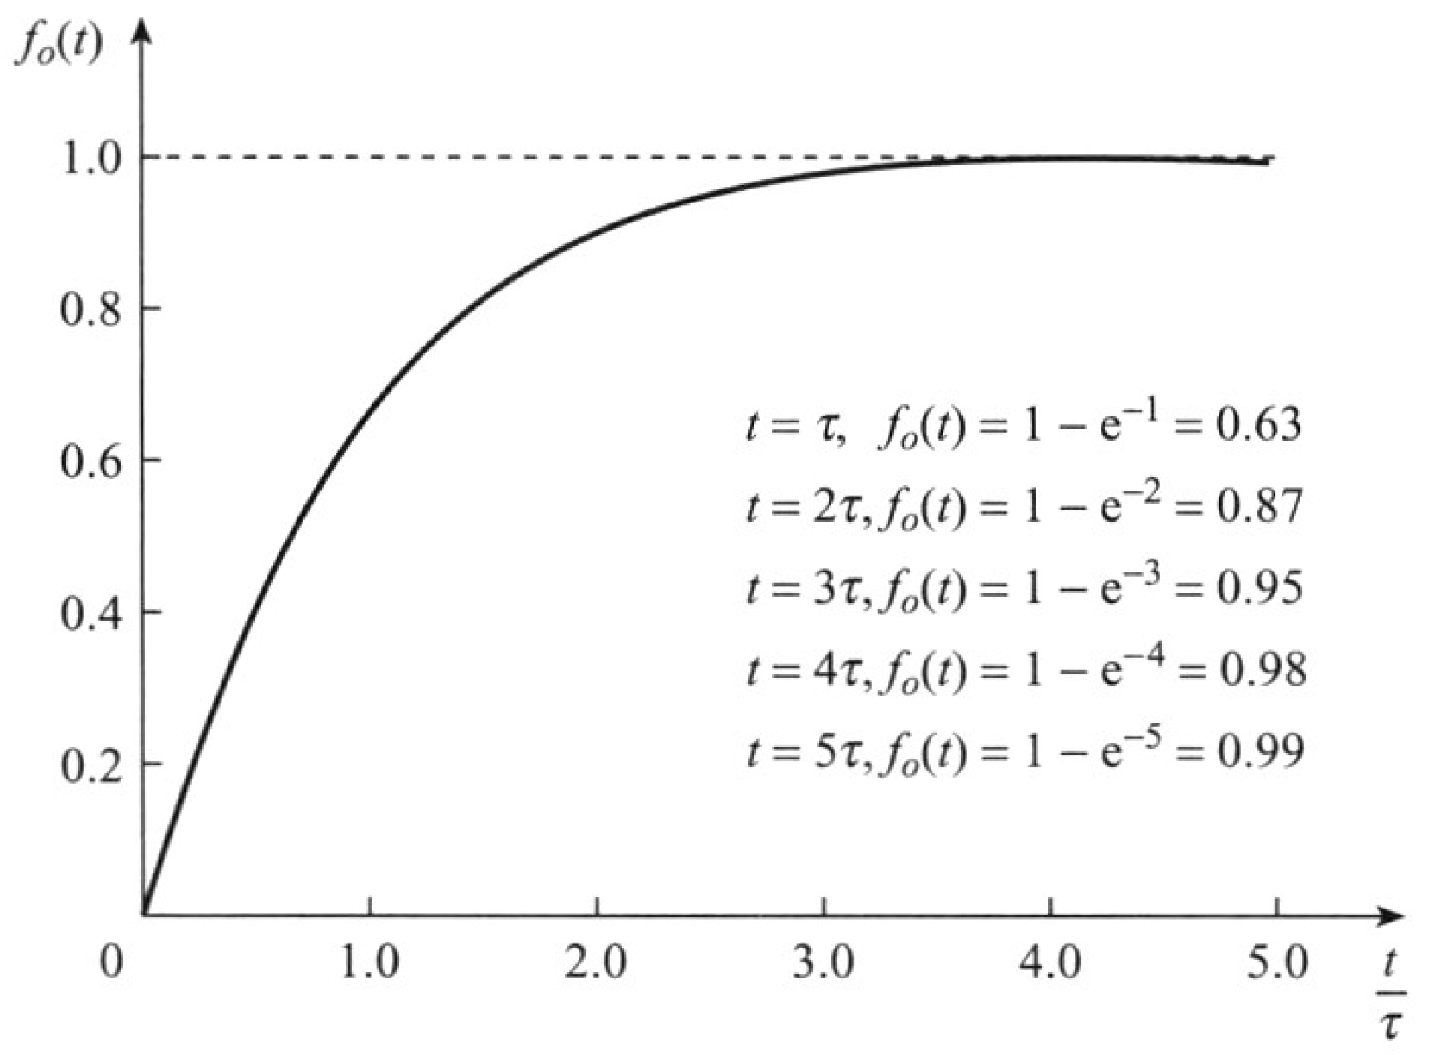
\includegraphics[scale=0.4]{./images/first-order-system-response.png}
\end{center}
\end{itemize}

 \newpage

\begin{itemize}
\item Second order
A second order system will behave in response to a step response as shown in the graph below:
\begin{center}
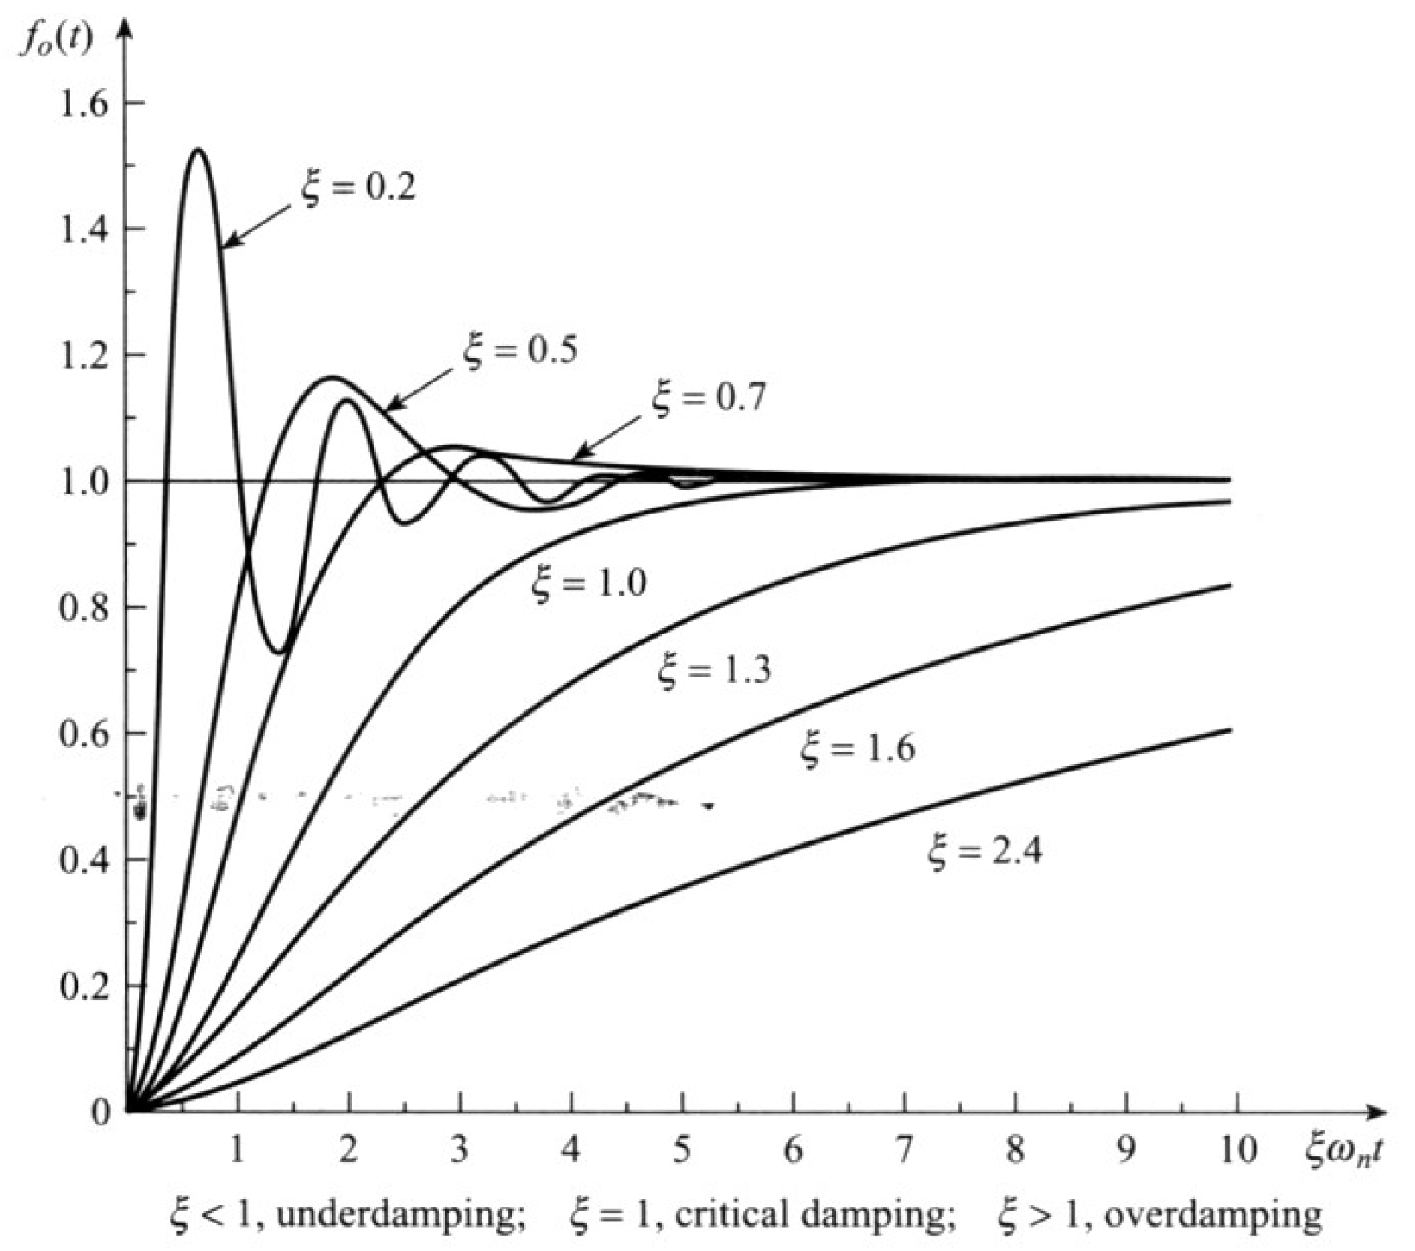
\includegraphics[width=.9\linewidth]{./images/second-order-system-response.png}
\end{center}
\end{itemize}

 \newpage
\subsection{Input signal conditional and interfacing}
\label{sec:org408559d}

\subsubsection{Discrete circuits}
\label{sec:org8e6549d}
Discrete circuits are circuits made up of discrete components, like resistors, capacitors, etc.
\subsubsection{Amplifiers}
\label{sec:orgcaa4e76}
Amplifiers amplify the signal to improve signal-to-noise ratio (SNR).
\subsubsection{Filters}
\label{sec:org0c576d1}
Filters get rid of unwanted signal contents, e.g. high-pass, low-pass, band-pass, band-stop, etc.
\subsubsection{Analogue to digital converter}
\label{sec:orgdcfd720}
Analogue to digital converters convert analogue signals like the turning of a knob, into a digital signal.
\subsection{Output signal conditioning and interfacing}
\label{sec:orgcc63428}
\begin{itemize}
\item Filters
\item Output amplifiers
\item Digital to analogue converter (DAC)
\item Etc.
\end{itemize}
\subsection{Graphical displays}
\label{sec:org285328a}
\begin{itemize}
\item Light Emitting Diodes (LED)
\item Liquid Crystal Display (LCD)
\end{itemize}

 \newpage
\subsection{Digital control architectures}
\label{sec:org19772a7}
\begin{itemize}
\item The digital control architecture is the "brain" of the system, and is usually a microcomputer.
\item Microprocessor (MPU) refers to the Central Processing Unit (CPU) on a single integrated-circuit (IC) chip.
\item Microcomputer refers to the MPU combined with the memory (RAM) and input and output unit (I/O unit)
\item Microcontroller (MCU) refers to the microcomputer in a single integrated-circuit (IC) chip.
\item Function: Logic, Arithmetic, Control, Timing and Sequencing, Communications, etc.
\end{itemize}

 \newpage
\section{Basic computer structure}
\label{sec:orgdcd44da}
All computers contain 3 basic units.

\begin{center}
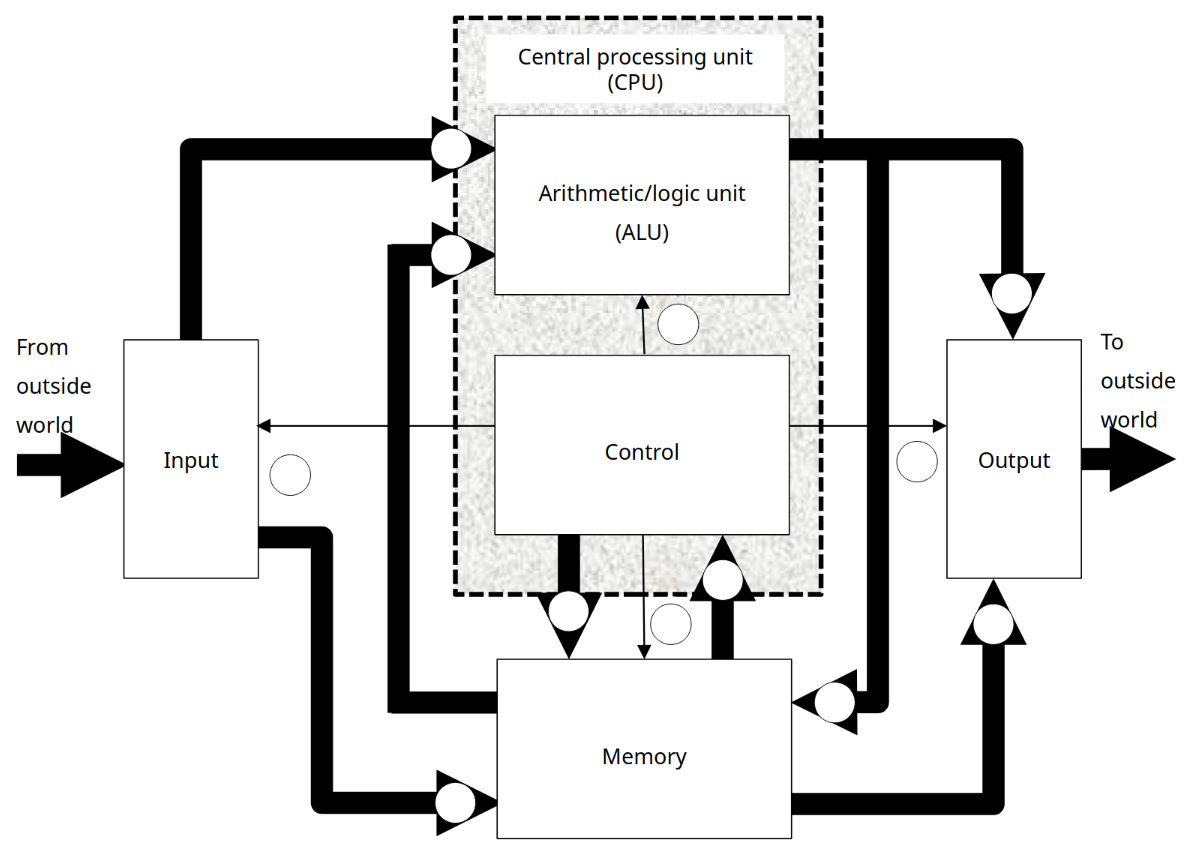
\includegraphics[width=.9\linewidth]{./images/basic-computer-structure.png}
\end{center}
\subsection{Central Processing Unit (CPU)}
\label{sec:org330cced}
\begin{itemize}
\item Arithmetic and Logic Unit (ALU)
\item Control Unit
\end{itemize}
\subsection{Memory Unit}
\label{sec:org571eb02}
\begin{itemize}
\item Internal memory, like Random Access Memory (RAM), Read-only Memory (ROM).
\item External memory, like Hard Disk Drives (HDD), Cassette Tape, etc.
\end{itemize}
\subsection{Input/Output Unit (I/O Unit)}
\label{sec:org0e9aa10}
\begin{itemize}
\item Input unit - Mouse, keyboard (K/B), Analogue to Digital Converter (ADC)
\item Output unit - Display, Digital to Analogue Converter (DAC)
\end{itemize}
\section{Design tips for mechatronics systems}
\label{sec:org42b0cfe}
\begin{enumerate}
\item Understand the task and define the problem
\item Sketch a function block diagram
\item Decide and select mechatronics components (type, number, communication protocol, etc.):
\begin{itemize}
\item Digital control architecture
\item Sensors and input interfacing
\item Actuators and output interfacing
\item Display
\end{itemize}
\item Look for the components with suitable specifications and ensure compatibility of components when they interface with each other
\item Construct hardware prototypes
\item Program software or firmware
\end{enumerate}
\section{Examples of mechatronics systems}
\label{sec:org0db7211}

\subsection{Car}
\label{sec:org7f396f0}
A typical car contains over 50 microprocessors for the systems listed below:
\begin{itemize}
\item Fuel and fluid alert system
\item Airbag system
\item Entertainment and navigation systems
\item Speed control system
\item Combustion engine control
\item Automatic gearbox
\item Active stabilisation
\item Anti-lock braking system (ABS)
\item Climate control (air-conditioning)
\item Seatbelt alert system
\item Door security system
\end{itemize}
\subsection{Inkjet printer}
\label{sec:org53d5099}

\subsubsection{Actuators}
\label{sec:org7321ebd}
\begin{itemize}
\item Stepper motor to drive print head mechanism
\item Stepper motor to drive paper feeding mechanism
\item Stepper motor to park print head mechanism (some models)
\item Ink firing at nozzles
\begin{itemize}
\item Piezoelectric (Epson) or Thermal resistor (Canon and HP)
\end{itemize}
\end{itemize}
\subsubsection{Sensors in paper feeding mechanism}
\label{sec:org47804ee}
\begin{itemize}
\item Proximity sensors or limit switch to detect presence of paper
\item Proximity sensors to detect paper loaded in position at the start of a print
\end{itemize}
\subsubsection{Sensors in print head mechanism}
\label{sec:org33a0f83}
\begin{itemize}
\item Linear encoder for precision positioning of print head
\item Limit switch to detect print head in parked position
\end{itemize}
\subsubsection{Digital control architecture}
\label{sec:org881f3b8}
\begin{itemize}
\item Microcontroller based
\item Communications
\begin{itemize}
\item USB (parallel) port
\item Bluetooth
\item Local Area Network (LAN) port
\item Wi-Fi
\end{itemize}
\item Graphics display is a simple LCD to high definition LED
\end{itemize}
\subsection{Robots}
\label{sec:org526d850}
\begin{itemize}
\item Serial robot
\item Parallel robot
\end{itemize}
\section{Sensors}
\label{sec:orgfbf3431}

\subsection{Digital sensors}
\label{sec:org96515f7}

\subsubsection{Switches}
\label{sec:org696f135}
\begin{center}
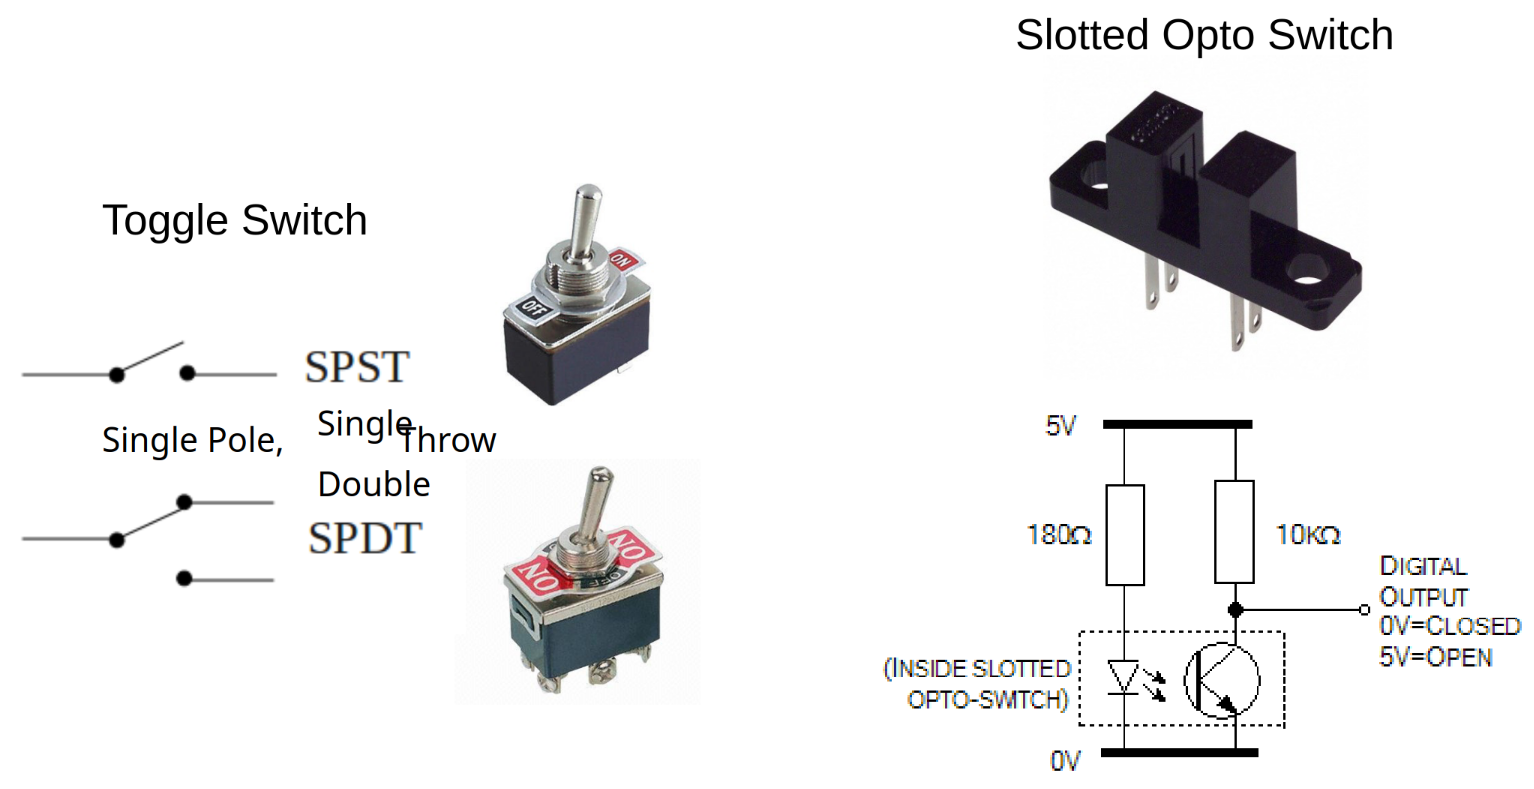
\includegraphics[width=.9\linewidth]{./images/toggle-and-slotted-opto-switches.png}
\end{center}
\begin{center}
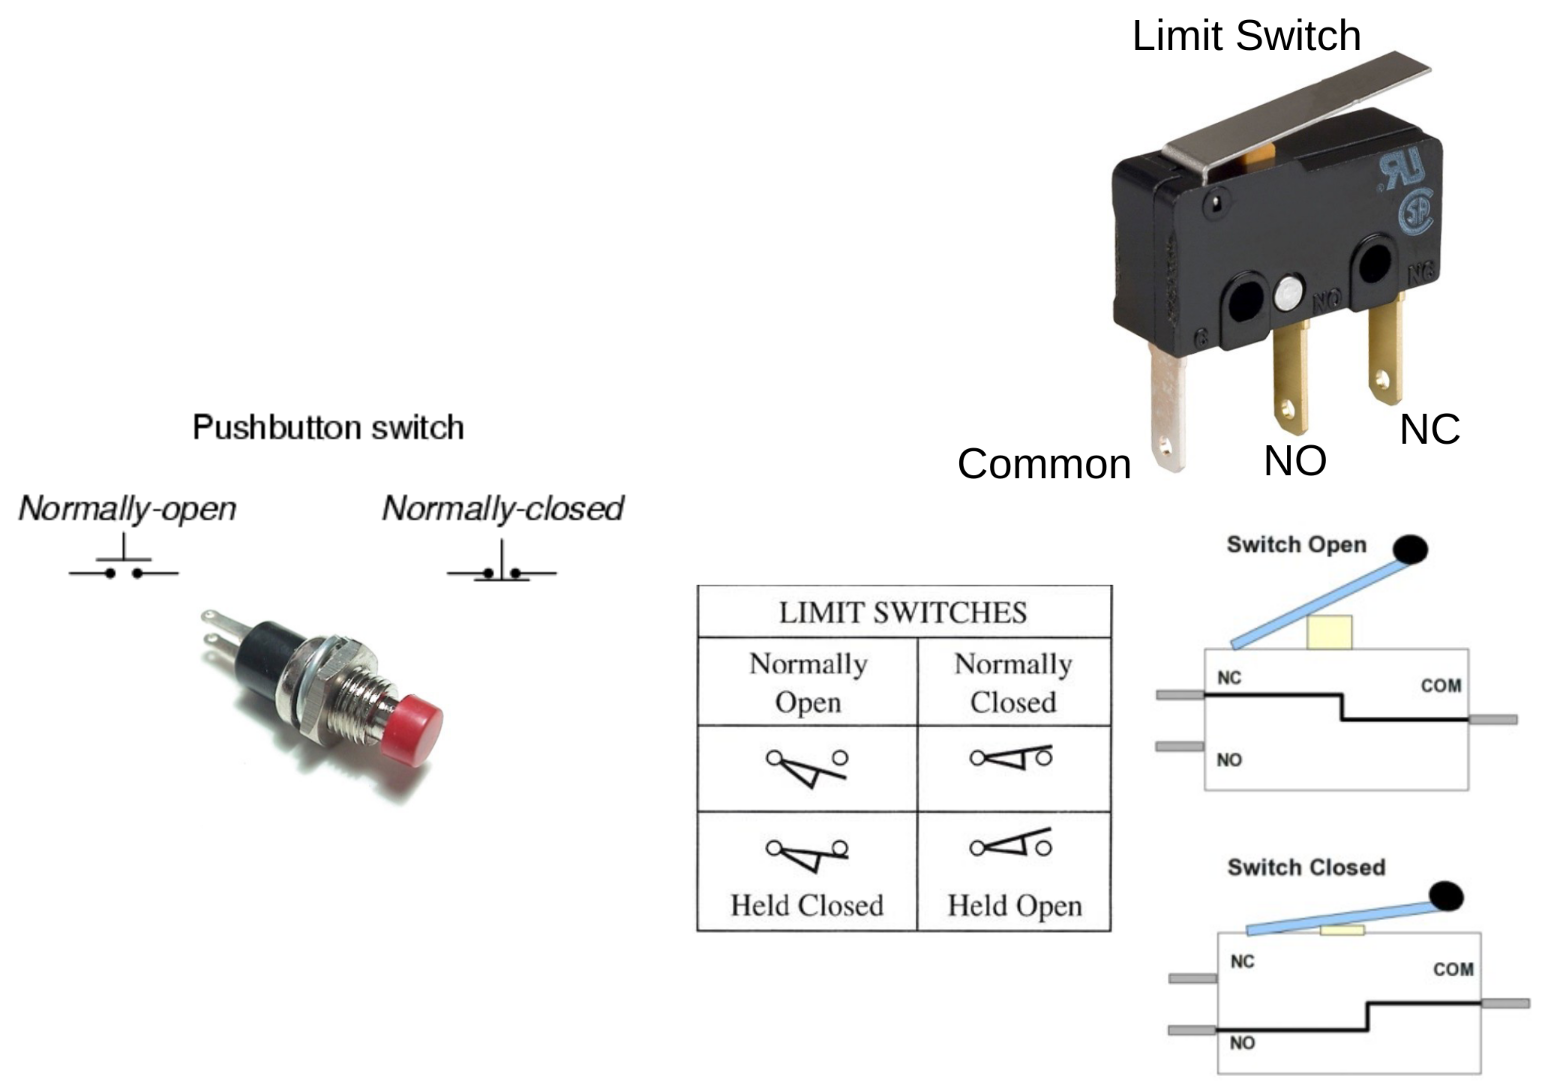
\includegraphics[width=.9\linewidth]{./images/pushbutton-and-limit-switches.png}
\end{center}

 \newpage
\subsubsection{Proximity sensor}
\label{sec:org73ed288}
A proximity sensor detects the presence of an object. Its output is either high, or low upon detection.
\begin{itemize}
\item Infrared and ultrasound sensors detect the incoming waves reflected by the object. An example is a car reverse sensor.
\item Inductive sensors change the induced current upon detection of ferrous or magnetic materials. An example is a metal detector for security.
\item Capacitive sensors change their capacitance upon detection of conductive materials. An example is a touch screen.
\end{itemize}

\begin{center}
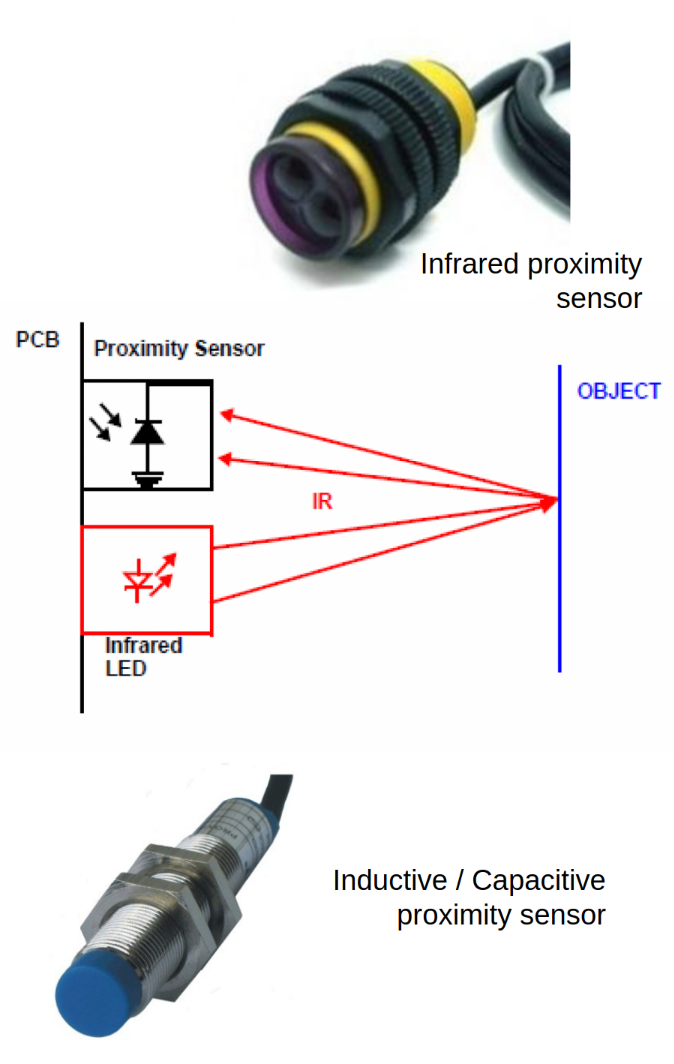
\includegraphics[scale=0.7]{./images/proximity-sensors.png}
\end{center}
\subsubsection{Incremental encoders}
\label{sec:org71c9b37}
\begin{center}
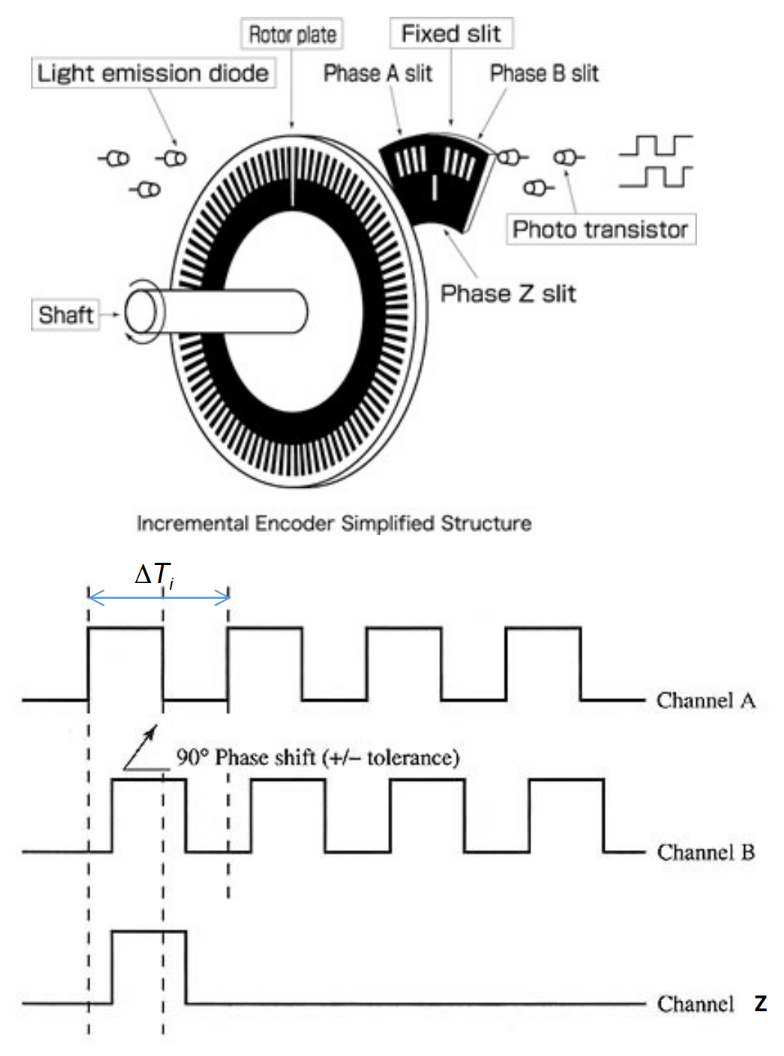
\includegraphics[scale=0.7]{./images/incremental-encoder.png}
\end{center}
Incremental encoders have the same working principle as the slotted opto switch.
\begin{itemize}
\item When channel A \textbf{leads} channel B by \(90^{\circ}\), the direction is anti-clockwise.
\item When channel A \textbf{lags} channel B by \(90^{\circ}\), the direction is clockwise.
\item The time \(\Delta T_i\) between 2 pulses determines the rotation speed, as:
\end{itemize}
\subsubsection{Digital encoders}
\label{sec:org2683065}
\begin{center}
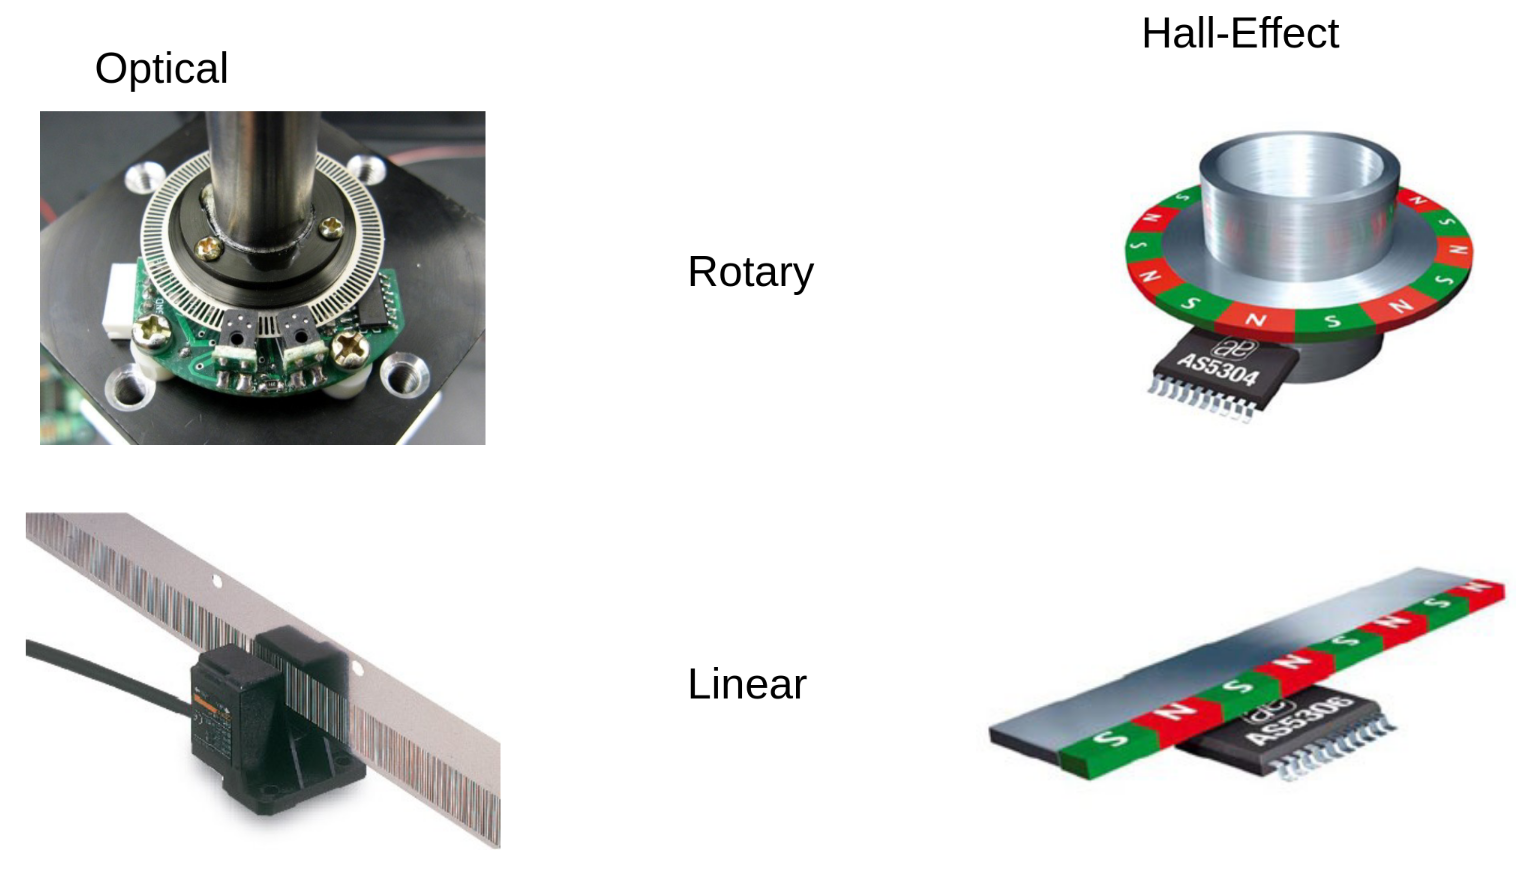
\includegraphics[width=.9\linewidth]{./images/digital-encoders.png}
\end{center}
  \[\omega_i = \frac{2 \pi}{\Delta T_i}\]
\subsection{Interfacing with digital sensors}
\label{sec:orge232851}

\subsubsection{Sensing modalities}
\label{sec:org9af6591}
\begin{itemize}
\item One modality is to sense a state, like high (1) or low (0).
\item Another modality is to measure the time duration of a state.
\end{itemize}
\subsubsection{Communication protocols}
\label{sec:org71be9df}
\begin{itemize}
\item Serial, where data is fed one after another.
\begin{itemize}
\item There are two types of serial communication, synchronous and asynchronous.
\item Serial is cheaper but slower
\end{itemize}
\item Parallel, where multiple streams of data is fed via multiple I/O pins.
\begin{itemize}
\item It is more expensive, but also faster.
\end{itemize}
\end{itemize}

 \newpage
\subsection{Analogue sensors}
\label{sec:org876c3a4}

\subsubsection{Potentiometer}
\label{sec:orgd2a107d}
\begin{itemize}
\item A potentiometer is used to measure angular or linear displacement.
\item It works based on the voltage divider principle where:
\[\text{Variable resistance} \propto \text{Variable voltage}\]
\item Applications of potentiometers include light dimmers and the knob to adjust the audio volume.
\end{itemize}

\begin{center}
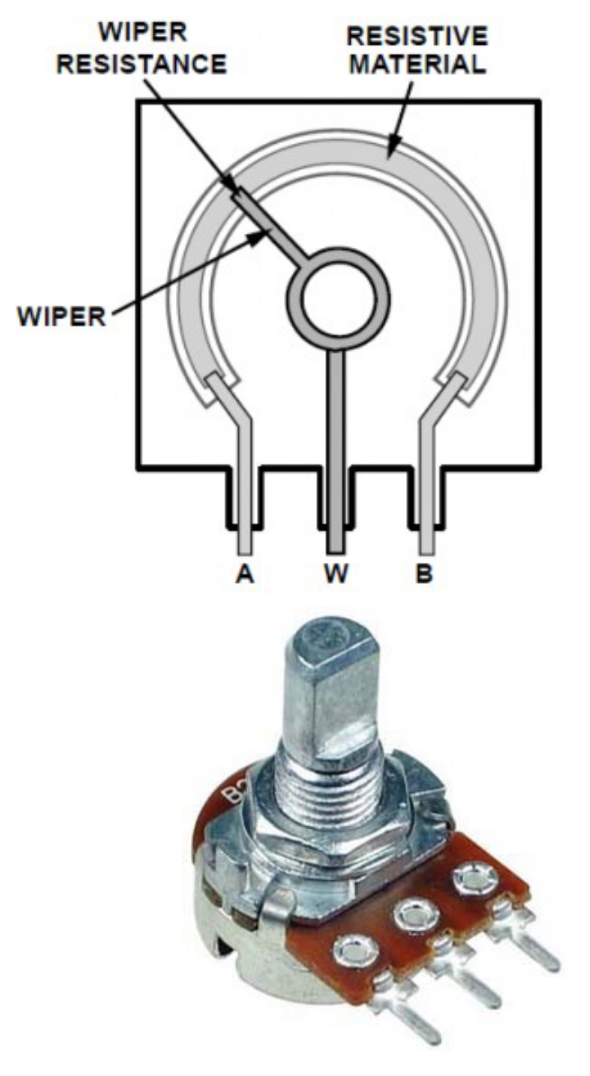
\includegraphics[scale=0.5]{./images/potentiometer-diagram.png}
\end{center}

\begin{center}
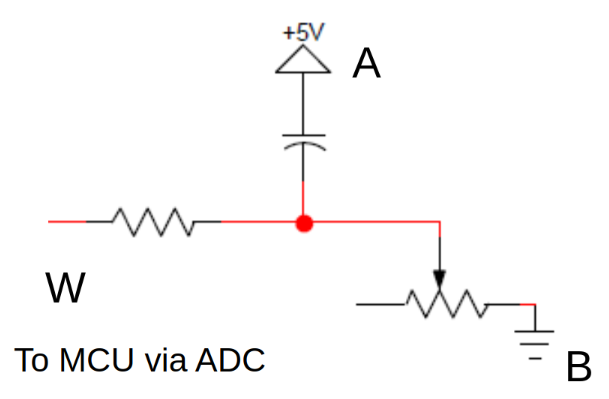
\includegraphics[scale=0.5]{./images/potentiometer-circuit.png}
\end{center}
\subsubsection{Accelerometer}
\label{sec:orgb5688a1}
\begin{itemize}
\item An accelerometer is used to measure linear acceleration from movement and gravity.
\item For an analogue accelerometer, its output is a voltage value.
\item For a digital accelerometer, its output is a duty cycle.
\item It works because motion causes a change in the distance between the plates and hence a change in the capacitance of the accelerometer.
\item Applications of accelerometers include mobile devices and inclinometer, which is an instrument used for measuring angles of slope, elevation, or depression with respect to gravity's direction.
\end{itemize}

\begin{center}
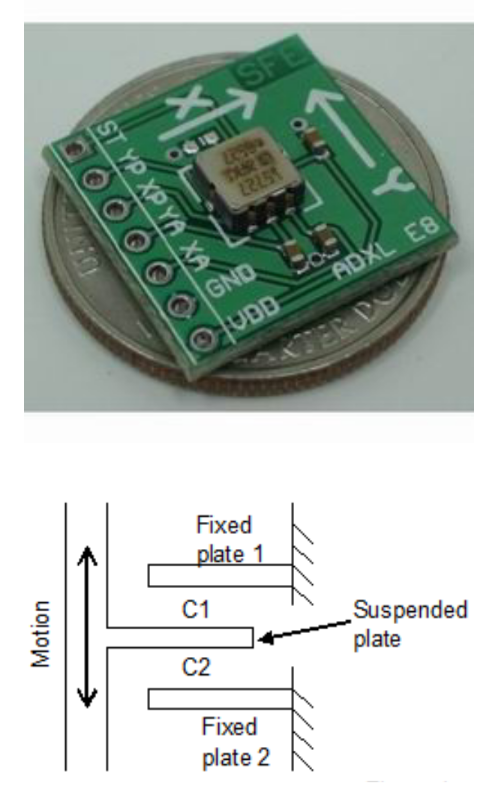
\includegraphics[scale=0.9]{./images/accelerometer-diagram.png}
\end{center}
\section{Analogue to digital converters}
\label{sec:orgc25626b}

\subsection{Successive approximation}
\label{sec:orgf16d2c9}
Successive is a fast, cheap and the most widely used method to convert analogue signals to digital signals.


The steps to convert an analogue signal to a digital signal using successive approximation:
\begin{enumerate}
\item With a start signal, analogue input is temporarily stored at the sample and hold (S\&H) latch.
\item The control unit makes an approximation of a digital equivalent of the analogue input and hold the result at an output latch.
\item The digital to analogue convert converts the digital approximation to analogue signal compares it with the analogue input.
\item If both are equal, the result held at the latch is the output. Otherwise, it goes back to step 2 to make the next successive approximation iteration.
\end{enumerate}

\begin{center}
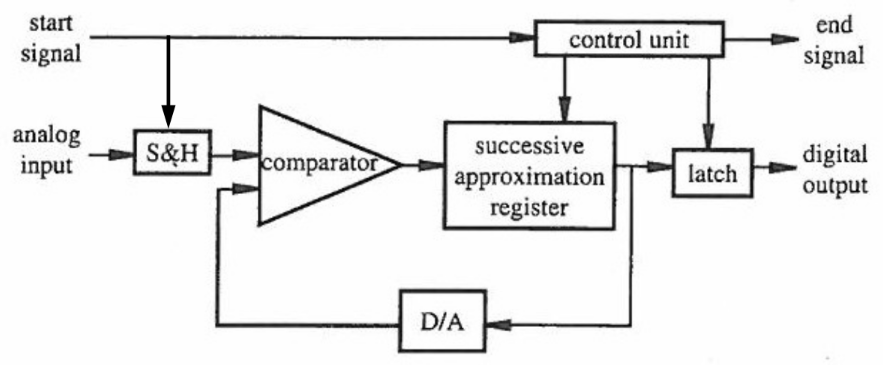
\includegraphics[width=.9\linewidth]{./images/successive-approximation.png}
\end{center}
\subsubsection{Example}
\label{sec:orgc2d40ce}
\begin{center}
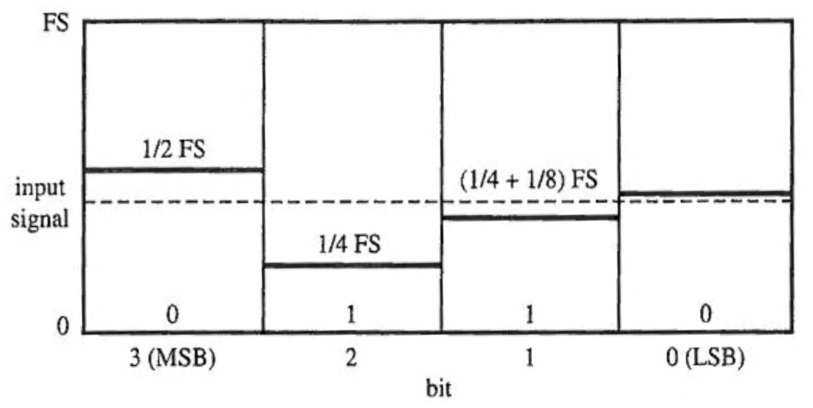
\includegraphics[scale=0.7]{./images/successive-approximation-example.png}
\end{center}

\begin{itemize}
\item Full Scale (\(FS\)) is \(\qty{1.0}{V}\)
\item Resolution (\(n\)) is 4 bits
\item Analogue input is \(\qty{0.4}{V}\)
\end{itemize}

Steps:
\begin{enumerate}
\item Control unit turns on only the most significant bit (MSB), which is Bit 3, that represents \(\frac{1}{2} FS = \qty{0.5}{V}\). The first approximation is 1000 in binary.
\item It is larger than the analogue input given (\(\qty{0.4}{V}\)), hence Bit 3 is turned off.
\item Control unit turns on Bit 2 \(\frac{1}{4} FS = \qty{0.25}{V}\). The second approximation is 0100 in binary.
\item Current value of \(\qty{0.25}{V} < \qty{0.4}{V}\), hence Bit 2 remains on.
\item Control unit turns on Bit 1 \(\frac{1}{8} FS = \qty{0.125}{V}\). The third approximation is 0110 in binary.
\item Current value of \(\qty{0.25}{V} + \qty{0.125}{V} = \qty{0.375}{V} < \qty{0.4}{V}\). Bit 1 remains on.
\item Control unit turns on Bit 0 \(\frac{1}{16} FS = \qty{0.0625}{V}\). The fourth approximation is 0111 in binary.
\item Current value of \(\qty{0.375}{V} + \qty{0.0625}{V} = \qty{0.4375}{V} > \qty{0.4375}{V}\). Bit 0 is turned off.
\item Final output is 0110 in binary, which is \(\qty{0.375}{V}\).
\end{enumerate}
\subsection{Flash converter}
\label{sec:orgad2a12b}
\begin{itemize}
\item A flash converter is a series of comparators acting in parallel to approximate an analogue input.
\item Fastest type of analogue-to-digital converter.
\item Increasing resolution does not increase conversion time.
\item Flip-flop latches produce 3-bit code.
\item AND \& OR gates to convert 3-bit code to binary output.
\end{itemize}

\begin{center}
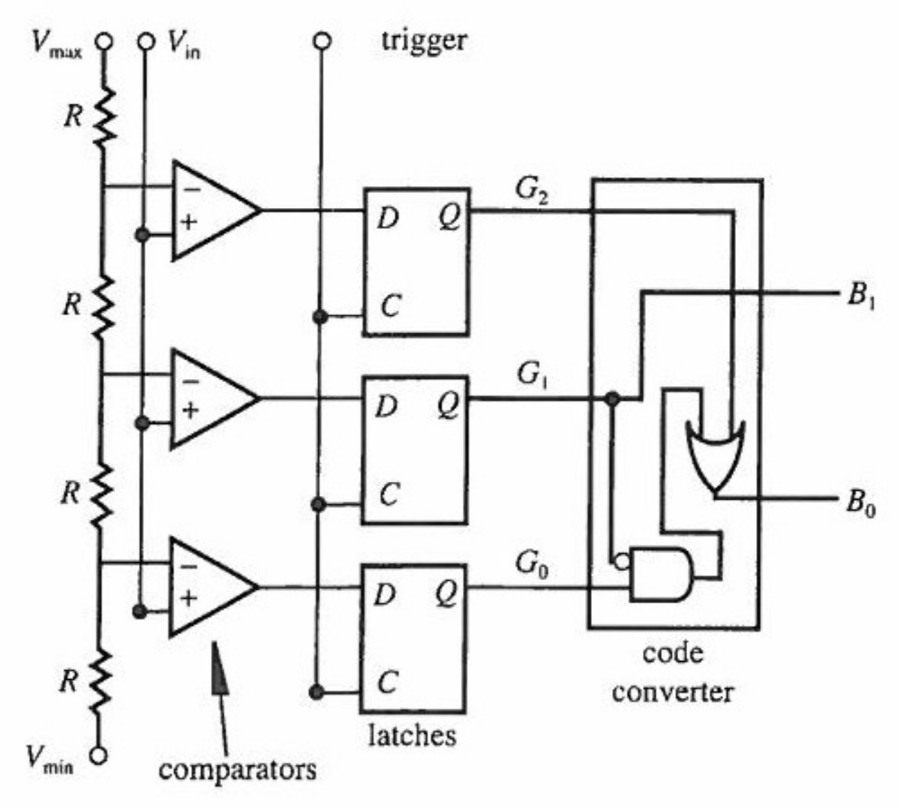
\includegraphics[width=.9\linewidth]{./images/flash-converter.png}
\end{center}

\begin{center}
\begin{tabular}{r|r|r|l}
State & Code (G\textsubscript{2} G\textsubscript{1} G\textsubscript{0}) & Binary (B\textsubscript{1} B\textsubscript{0}) & Voltage Range (V)\\
\hline
0 & 000 & 00 & 0 to 1\\
1 & 001 & 01 & 1 to 2\\
2 & 011 & 10 & 2 to 3\\
3 & 111 & 11 & 3 to 4\\
\end{tabular}
\end{center}

\[B_0 = G_0 \cdot G_1 + G_2\]
\[B_1 = G_1\]
\section{Data acquisition (DAQ) process}
\label{sec:org1e1e1a2}
\begin{center}
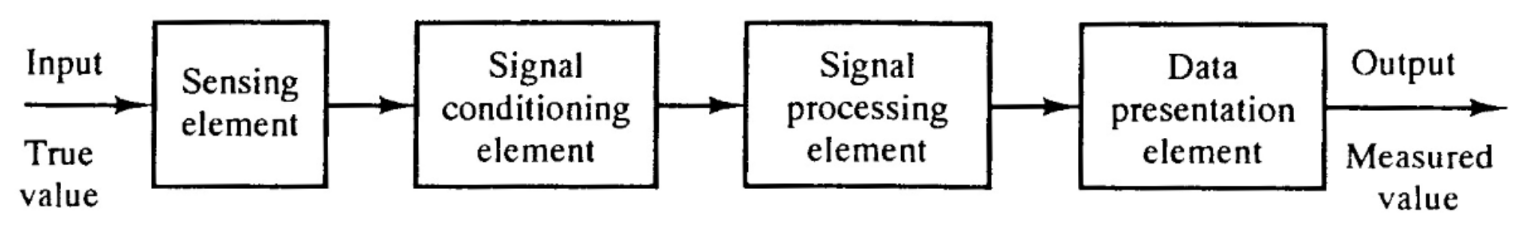
\includegraphics[width=.9\linewidth]{./images/data-acquisition-process.png}
\end{center}
\subsection{Sensing element}
\label{sec:org0f7a107}
The sensing element is the element in contact with the process and gives an output which depends in some ways on the variables to be measured.

Examples:
\begin{itemize}
\item Thermocouple: Measured E.M.F in \(\unit{mV}\) depends on temperature.
\item Strain gauge: Its resistance depends on mechanical strain.
\end{itemize}
\subsection{Signal conditioning element}
\label{sec:orgd6642af}
The signal conditioning element takes the output of the sensing element and converts it into a form more suitable for further processing, usually a DC voltage, a DC current or frequency signal.

Examples:
\begin{itemize}
\item An amplifier which amplifies \(\unit{mV}\) to \(\unit{V}\).
\item Wheatstone bridge that converts impedance change into voltage change.
\end{itemize}
\subsection{Signal processing element}
\label{sec:orgf7eb897}
The signal processing element takes the output of the signal conditioning element and converts it into a form more suitable for presentation.

Examples:
\begin{itemize}
\item Analogue-to-Digital converter which converts a voltage into a digital form.
\item Computer which calculates the desirable measurement from raw data, like:
\begin{itemize}
\item The mass of gas from flow rate and density.
\item Correction for non-linearity.
\end{itemize}
\end{itemize}
\subsection{Data presentation element}
\label{sec:orgb4f7c6b}
The data presentation element presents the measured value in a form which can be easily recognised by the observer.

Examples:
\begin{itemize}
\item Visual Display Unit (VDU)
\item Dial or pointer-scale indicator
\end{itemize}
\subsection{Examples of the DAQ process}
\label{sec:org9a448c3}
\begin{center}
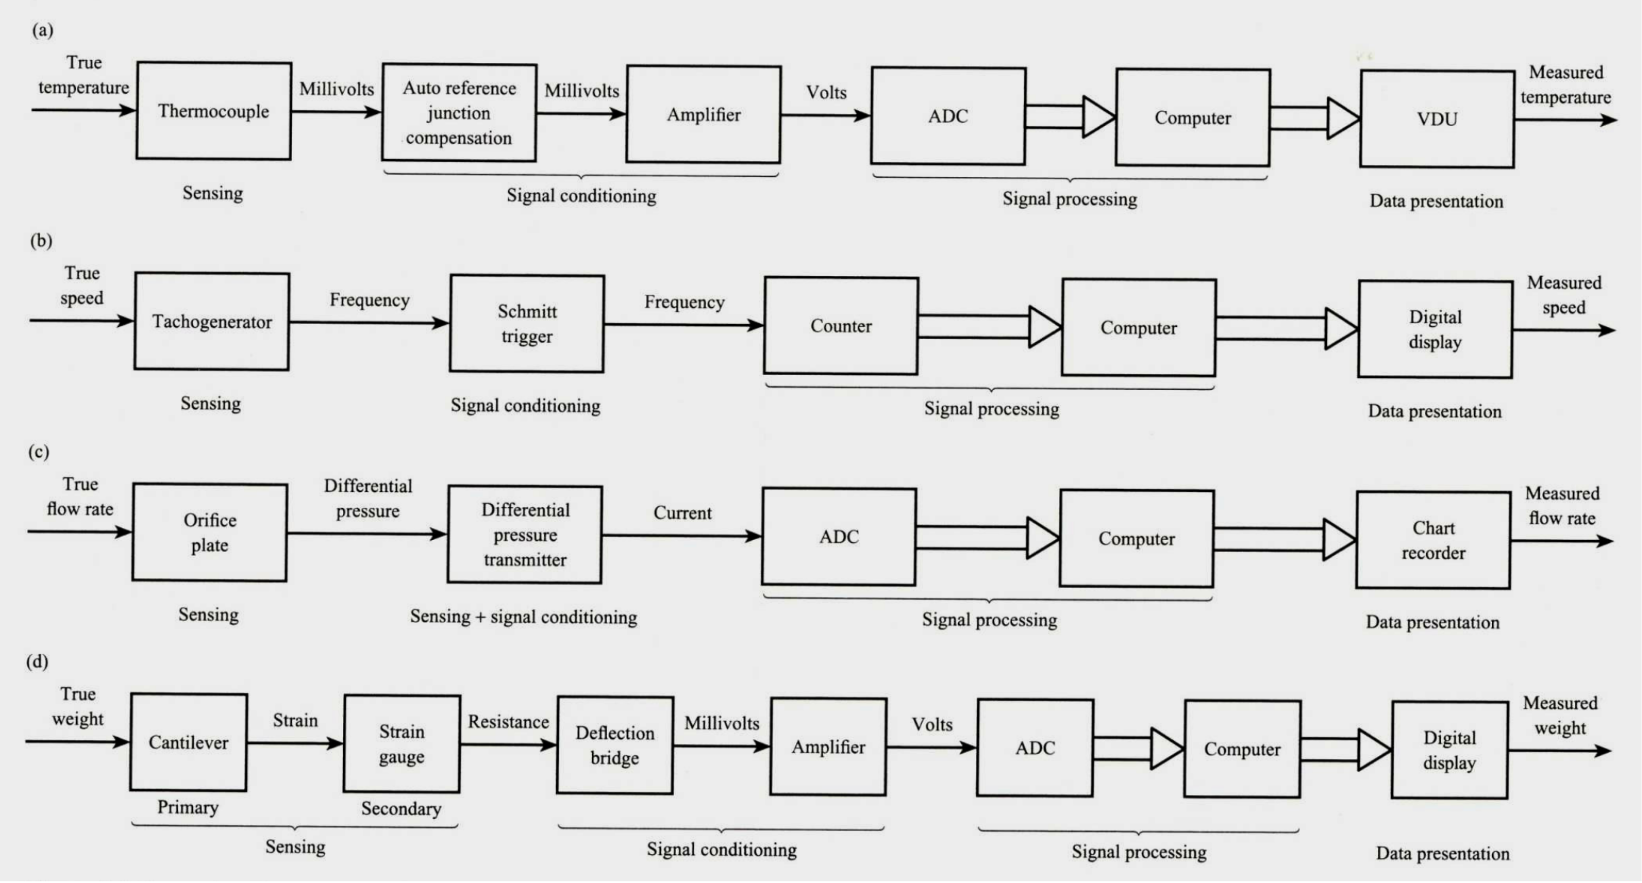
\includegraphics[width=.9\linewidth]{./images/data-acquisition-process-examples.png}
\end{center}

 \newpage
\section{Direct current motor}
\label{sec:orgf07dcad}

\subsection{Permanent magnet or brushed DC motors}
\label{sec:org6b83f5c}
\begin{itemize}
\item The stator, which is the external shell containing the components of the DC motor, is fixed in place.
\item The rotor, which is the rotating internal part inside the stator, rotates to produce the movement.
\item The motor works based on Fleming's left-hand rule.
\end{itemize}

\begin{center}
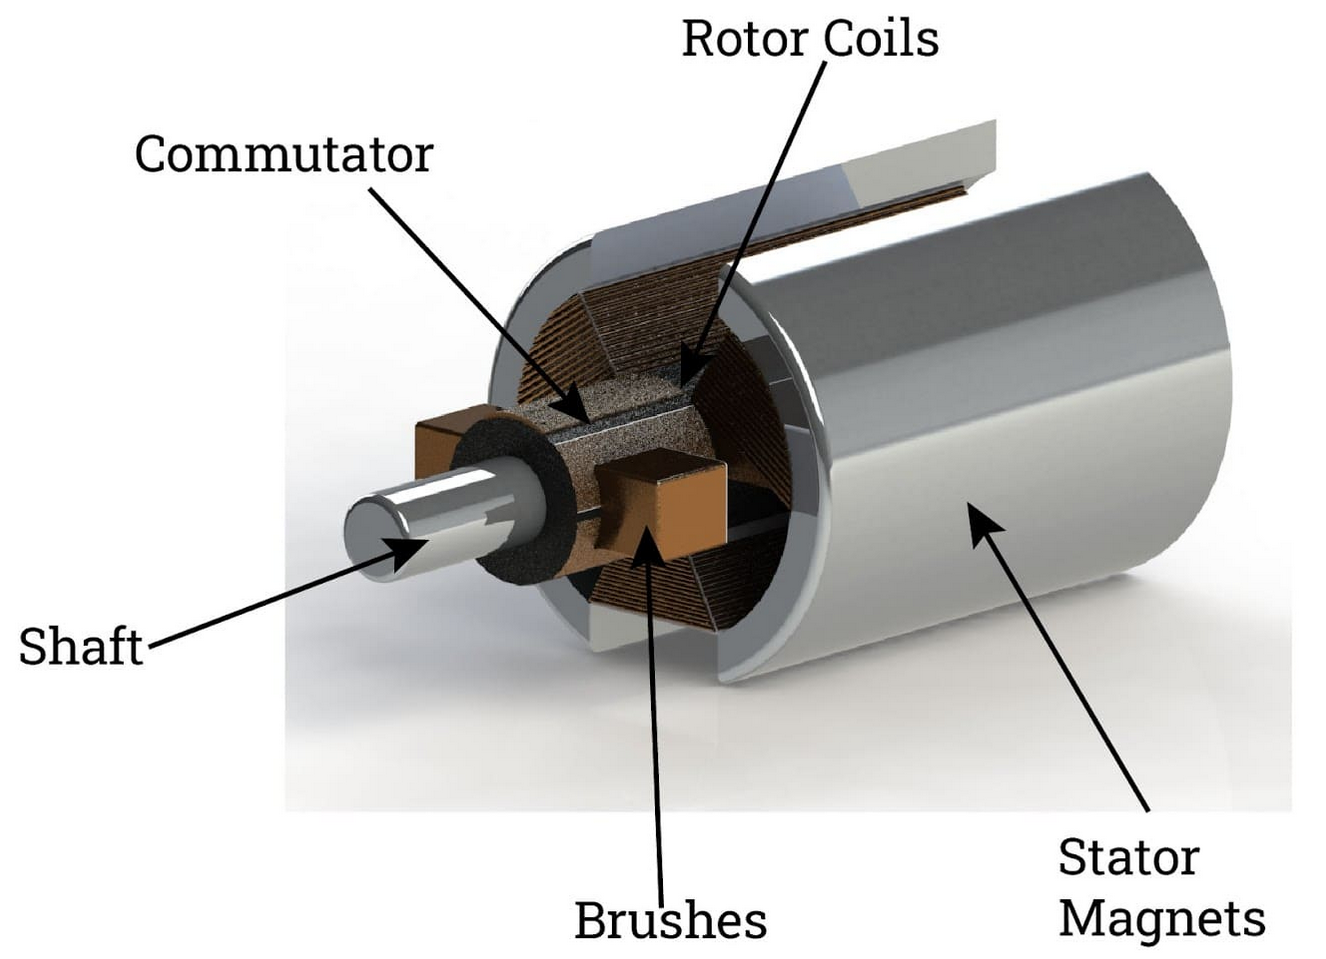
\includegraphics[width=.9\linewidth]{./images/brushed-dc-motor.png}
\end{center}

 \newpage
\subsection{Brushless DC motor}
\label{sec:orga4d19d6}
\begin{itemize}
\item It has the same body as a brushed DC motor, with a permanent magnet rotor on the inside and a fixed stator with rotating magnetic fields.
\item It needs to know the exact angular position of the rotor to excite the correct coils. This is usually done with Hall effect sensors.
\end{itemize}

\begin{center}
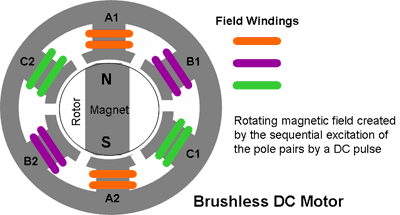
\includegraphics[width=.9\linewidth]{./images/brushless-dc-motor-diagram.png}
\end{center}
\begin{center}
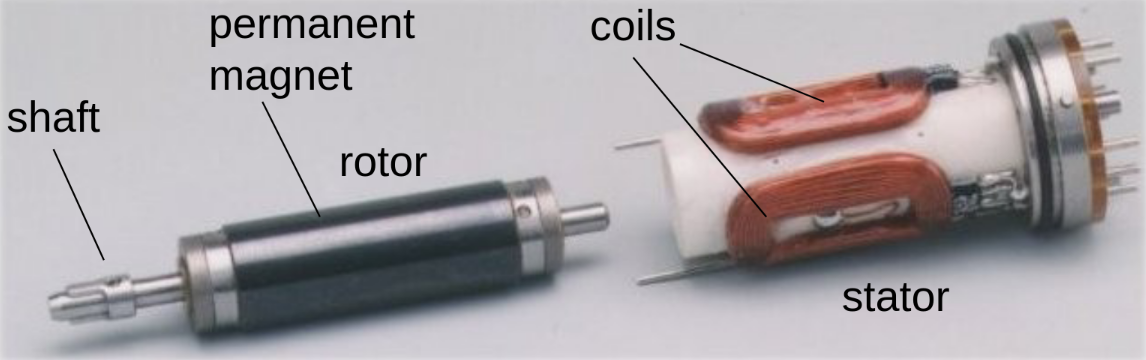
\includegraphics[width=.9\linewidth]{./images/brushless-dc-motor.png}
\end{center}
\subsection{Brushless vs brushed DC motors}
\label{sec:org995d7a4}
\begin{center}
\begin{tabular}{m{16em}|m{16em}}
Brushless & Brushed\\
\hline
Simple maintenance & Low cost thanks to the simple construction and control, and only two wires are needed.\\
\hline
High efficiency as there is no drop in voltage across the brush, and has low electrical noise & More robust in harsh environments as there are no electronic components\\
\hline
Higher speed range & \\
\hline
Reduced size & \\
\end{tabular}
\end{center}
\subsection{Controlling DC motors}
\label{sec:org2511169}
\begin{center}
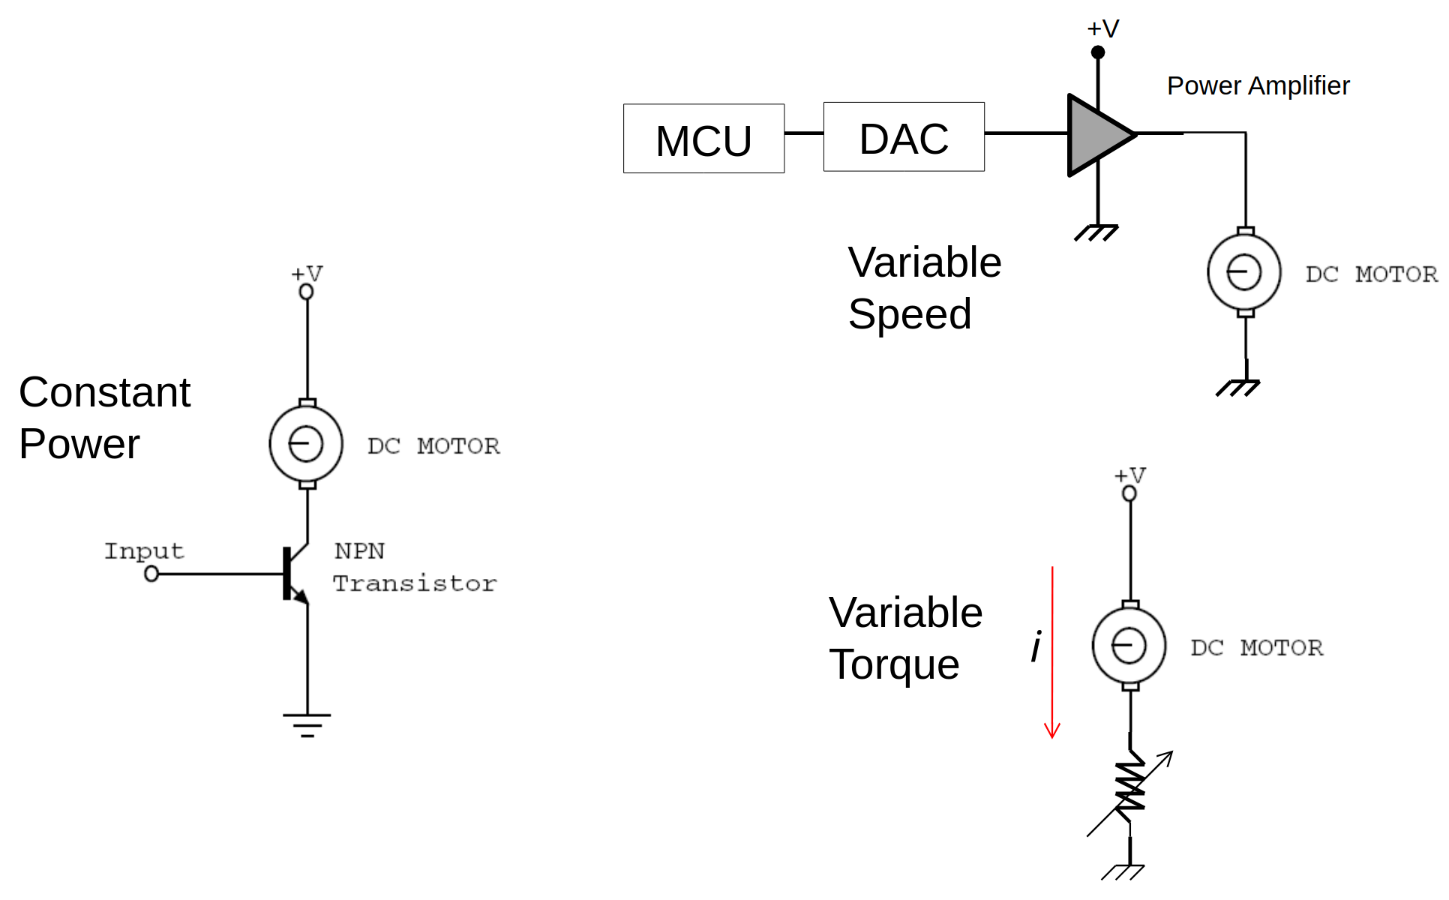
\includegraphics[width=.9\linewidth]{./images/controlling-dc-motors.png}
\end{center}
\subsubsection{Motion control fundamentals}
\label{sec:org4cc2e0d}
\begin{itemize}
\item Power \(= VI = \tau \omega\)
\item DC motor control
\begin{itemize}
\item Voltage controls velocity: \(V \propto \omega\)
\item Current controls torque: \(I \propto \tau\)
\end{itemize}
\end{itemize}
\subsubsection{Power amplifiers}
\label{sec:org31a133c}
Using power amplifiers is possible but is typically avoided. There is usually large power dissipation, and the amplifier usually overheats.
\subsubsection{Digital-to-analogue converter}
\label{sec:org3f9a034}
Digital to analogue converters (DACs) are expensive, so most MCUs are not equipped with a DAC.
\subsubsection{Uni-directional PWM control}
\label{sec:org80aa2a0}
\begin{center}
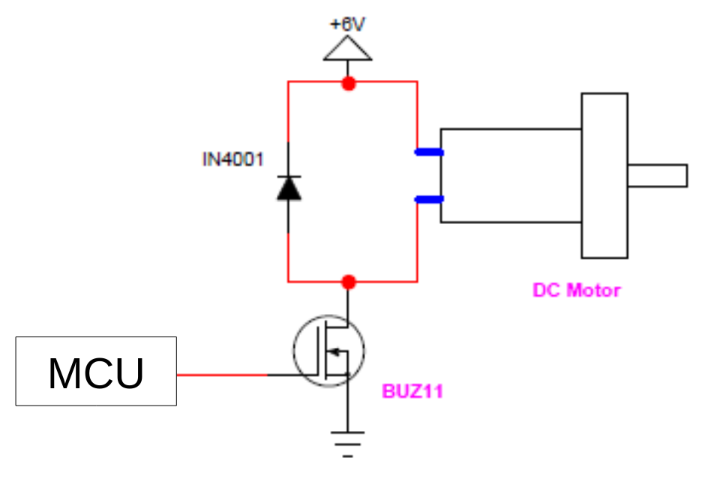
\includegraphics[width=.9\linewidth]{./images/uni-directional-pwm-control.png}
\end{center}
\subsubsection{Bidirectional PWM control}
\label{sec:orged1eac0}
Below is a bidirectional DC motor control using a dual power supply.

\begin{center}
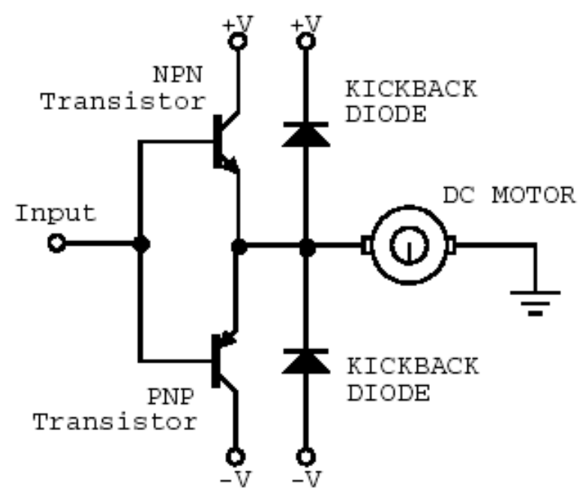
\includegraphics[scale=1]{./images/bidirectional-pwm-control.png}
\end{center}
\subsubsection{Bidirectional PWM control with H-bridge circuit}
\label{sec:orga0f717f}

\begin{center}
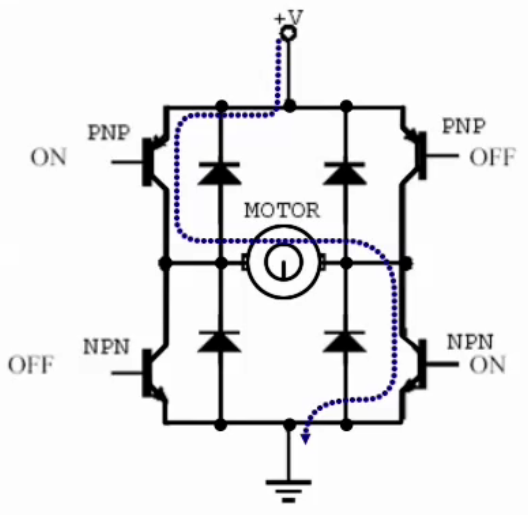
\includegraphics[width=0.49\textwidth]{./images/bidirectional-pwm-control-with-h-bridge-clockwise.png}
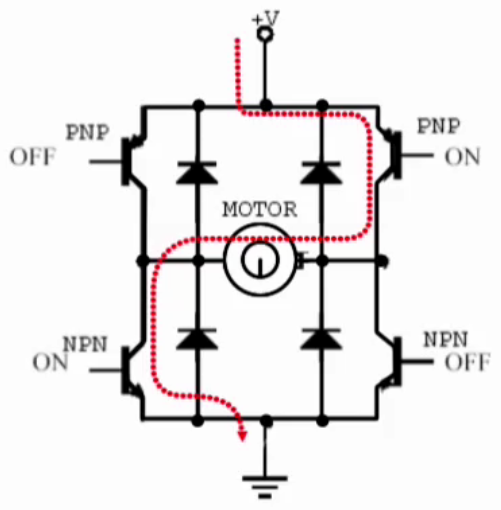
\includegraphics[width=0.49\textwidth]{./images/bidirectional-pwm-control-with-h-bridge-anti-clockwise.png}
\end{center}

\begin{center}
\begin{tabular}{>{\centering\arraybackslash}m{0.49\textwidth} >{\centering\arraybackslash}m{0.49\textwidth}}
Clockwise direction & Anti-clockwise direction\\
\end{tabular}
\end{center}
\section{Process and instrument control I/O}
\label{sec:org5e4a5a7}
\begin{itemize}
\item The microcontroller operates automatically and continuously under the control of the program stored in the ROM, no human intervention is required.
\begin{itemize}
\item The operation is changed only by changing the content of the ROM.
\end{itemize}
\item During execution, the microcontroller receives data from devices monitoring some physical states (temperature, speed, etc.), operates on the data and sends data or control signals to the process or instrument via output devices.
\end{itemize}
\subsubsection{Examples}
\label{sec:org7a21ec9}
\begin{itemize}
\item Traffic red-light camera
\item Car airbag system
\item Fire and burglar alarm systems
\end{itemize}

 \newpage
\section{Keyboard entry and display I/O}
\label{sec:org6b49481}
\begin{itemize}
\item Communication with human operators
\item The microcontroller executes a keyboard monitoring program stored in ROM.
\begin{itemize}
\item It reads the keyboard continuously until a key is actuated, then determines the actuated key, and executes the appropriate instructions.
\end{itemize}
\item Once the instructions are executed, it gets back to the keyboard monitoring program.
\end{itemize}
\subsubsection{Examples}
\label{sec:orgc4f6aeb}
\begin{itemize}
\item Point-of-sale machines
\item Lift
\item Television
\end{itemize}

 \newpage
\section{Deterministic and random signals}
\label{sec:org6346913}
\begin{center}
\includegraphics[scale=0.9]{./images/deterministic-vs-random-signals.png}
\end{center}
\subsection{Deterministic signals}
\label{sec:org9b41a51}
Deterministic signals are signals with values that can be predicted exactly, after an observation period \(T_0\).
\subsection{Random signals}
\label{sec:org06783dd}
Random signals are signals that cannot be predicted exactly, after an observation period \(T_0\). Essentially, the signal cannot be represented by a continuous algebraic equation \(y(t)\) for the signal \(y\) at time \(t\).
\subsection{Randomness}
\label{sec:orgdd2be30}
\begin{itemize}
\item A real process has many parameters that cannot be exactly known, because of the randomness of nature.
\item An absolutely clean signal does not exist if the resolution is allowed to be infinitesimally small.
\item Observed randomness is dependent on resolution.
\end{itemize}
\subsubsection{Leaves falling from a tree example}
\label{sec:orga05813e}
\begin{center}
\includegraphics[width=.9\linewidth]{./images/leaves-falling-from-a-tree-signal.png}
\end{center}

With a resolution of:
\begin{itemize}
\item \(\qty{1}{m^2}\), the outcome is noisy
\item \(\qty{100}{m^2}\), the outcome is clean
\end{itemize}

 \newpage
\subsubsection{Voltage source example}
\label{sec:org605a40c}
\begin{center}
\includegraphics[width=.9\linewidth]{./images/voltage-source-signal.png}
\end{center}

With a resolution of:
\begin{itemize}
\item \(\qty{0.1}{V}\), the outcome is clean
\item \(\qty{0.001}{V}\), the outcome is noisy
\end{itemize}
\section{Sources of noise}
\label{sec:org09979a8}

\subsection{Internal noise sources}
\label{sec:org80402e2}
\begin{itemize}
\item Johnson or thermal noise is random, temperature-induced motion of electrons and other charge carriers in resistors and semiconductors that give rise to a corresponding random voltage. The white noise is proportional to the absolute temperature in Kelvin (\(\unit{K}\)).
\item Shot noise is the random fluctuations in the rate at which charge carriers diffuse across a junction of a transistor. It is another source of white noise.
\end{itemize}

 \newpage
\subsection{External noise and interference sources}
\label{sec:org15fc961}
\begin{itemize}
\item AC power circuits operating at \(\qty{220}{V}, \qty{50}{Hz}\) (US: \(\qty{110}{V}, \qty{60}{Hz}\)) produce "mains pick-up" or "hum" which is a corresponding sinusoidal interference signal in the measurement circuit.
\item Fluorescent lighting arcing at 2 times per cycle of the AC power. Arcing is the process of raising the potential to cause electrical current to flow between the anode and cathode through the inert gases inside the tube of a fluorescent light.
\item Radio frequency (RF) interference. Transmitters, welding equipment and electric arc furnaces can produce interference at frequencies of several \(\unit{MHz}\).
\end{itemize}
\section{Input signal conditioning elements}
\label{sec:orga8c192f}
\begin{itemize}
\item Types of input signals that can be conditioned:
\begin{itemize}
\item DC voltage
\item DC current
\item Variable frequency AC voltage
\end{itemize}
\item Examples:
\begin{itemize}
\item Deflection bridges
\item Operational amplifiers (Op-Amp)
\item Filters
\end{itemize}
\end{itemize}
\subsection{Deflection bridges}
\label{sec:org5e89148}
\begin{itemize}
\item Deflection bridges measure the deflection of a material by using strain gauges that change their resistance when there is strain on the gauge.
\end{itemize}
\subsubsection{Quarter bridge}
\label{sec:org8819704}
\begin{center}
\includegraphics[width=.9\linewidth]{./images/quarter-bridge-deflection-bridge.png}
\end{center}

The voltage output is given by \(V_g\):
\[V_g = V_s \left(\frac{1}{1 + \frac{R_4}{R_1}} - \frac{1}{1 + \frac{R_3}{R_2}} \right)\]
\subsubsection{Half bridge}
\label{sec:org78718cb}
Half bridges have double the sensitivity of the quarter bridges.
\begin{center}
\includegraphics[width=.9\linewidth]{./images/half-bridge-deflection-bridge.png}
\end{center}
\subsubsection{Full bridge}
\label{sec:orga9719e3}
Compared to half bridges, full bridges simplify the equation used to calculate the voltage output, and their output is more linear.
\begin{center}
\includegraphics[width=.9\linewidth]{./images/full-bridge-deflection-bridge.png}
\end{center}

 \newpage
\subsection{Operation amplifiers (Op-Amp)}
\label{sec:orgf95da56}
\begin{itemize}
\item Operational amplifiers (op-amps) are used as the basic building blocks for instrumentation and power amplifiers.
\item Types of op-amps:
\begin{itemize}
\item Inverting
\item Non-inverting
\item Voltage follower
\item Voltage adder
\item Differential
\end{itemize}
\end{itemize}
\subsubsection{Inverting amplifier}
\label{sec:orgb8edb89}
The voltage input is being amplified by the ratio \(\frac{R_F}{R_{IN}}\) and is inverted.
\begin{center}
\includegraphics[width=.9\linewidth]{./images/inverting-amplifier.png}
\end{center}
\[V_{OUT} = \frac{-R_F V_{IN}}{R_{IN}}\]
\subsubsection{Non-inverting amplifier}
\label{sec:org4bce460}
\begin{center}
\includegraphics[width=.9\linewidth]{./images/non-inverting-amplifier.png}
\end{center}
\[V_{OUT} = \left(1 + \frac{R_F}{R_{IN}} \right)\]
\subsubsection{Voltage follower}
\label{sec:orgecf0518}
Voltage followers increase the current passing through them while keeping the voltage from the input.
\begin{center}
\includegraphics[width=.9\linewidth]{./images/voltage-follower.png}
\end{center}
\[V_{OUT} = V_{IN}\]
\subsubsection{Voltage adder}
\label{sec:org2e9c2d6}
Voltage adders add up all the input voltages and amplify the sum of the input voltage.
\begin{center}
\includegraphics[width=.9\linewidth]{./images/voltage-adder.png}
\end{center}
\[V_{OUT} = -R_F \left(\frac{V_1}{R_1} + \frac{V_2}{R_2} + \cdots + \frac{V_n}{R_n} \right)\]

 \newpage
\subsubsection{Differential amplifier}
\label{sec:org93b63c8}
\begin{itemize}
\item Differential amplifiers amplify the difference between two voltage inputs.
\item A useful application of differential amplifiers is in removing background noise from a person speaking, which is a type of interference called common mode interference.
\item The microphone picks up both the person's voice and the background noise, then another microphone picks up only the background noise.
\item The differential amplifier is then used to amplify the difference between the two signals from the microphones, resulting in a clean signal of the person's voice.
\end{itemize}

\begin{center}
\includegraphics[scale=0.8]{./images/differential-amplifier.png}
\end{center}

\begin{center}
\includegraphics[scale=0.8]{./images/differential-amplifier-alt.png}
\end{center}
\[V_{OUT} = \frac{R_F}{R_{IN}} \left(V_2 - V_1 \right)\]
\subsection{Filters}
\label{sec:orgbda6a51}
\begin{itemize}
\item A frequency selective filter is an element which transmit a certain selected range of frequencies and rejects all others.
\item An analogue filter is a network of resistors, capacitors and op amps to process continuous signals.
\item A digital filter is a computer programmed to process sampled values of a signal.
\item RC filters refer to filters that have both a resistor and a capacitor.
\end{itemize}

\begin{center}
\includegraphics[width=.9\linewidth]{./images/filtering-image.png}
\end{center}
\subsubsection{Low and high pass filters (RC filters)}
\label{sec:orgf283fa4}
\begin{center}
\includegraphics[width=.9\linewidth]{./images/low-and-high-pass-filters.png}
\end{center}

 \newpage
\subsubsection{Passive low pass filters}
\label{sec:org44a38e6}
Passive low pass filters block all frequencies \textbf{above} the cut-off frequency \(f_c\).
\begin{center}
\includegraphics[width=.9\linewidth]{./images/passive-low-pass-filter.png}
\end{center}
\[f_c = \frac{1}{2 \pi \tau} = \frac{1}{2 \pi RC}\]

 \newpage
\subsubsection{Active low pass filters}
\label{sec:orgfe1a258}
Active low pass filters behave exactly the same as passive ones, just that they increase the current passing through them as they have an op-amp in the circuit. They also block all frequencies \textbf{above} the cut-off frequency \(f_c\).
\begin{center}
\includegraphics[width=.9\linewidth]{./images/active-low-pass-filter.png}
\end{center}
\[f_c = \frac{1}{2 \pi R_2 C}\]

 \newpage
\subsubsection{Passive high pass filters}
\label{sec:orgd8f3a6f}
Passive high pass filters block all frequencies \textbf{below} the cut-off frequency \(f_c\).
\begin{center}
\includegraphics[width=.9\linewidth]{./images/passive-high-pass-filter.png}
\end{center}
\[f_c = \frac{1}{2 \pi \tau} = \frac{1}{2 \pi RC}\]

 \newpage
\subsubsection{Active high pass filters}
\label{sec:org22f0e6e}
Active low pass filters behave exactly the same as passive ones, just that they increase the current passing through them as they have an op-amp in the circuit. They also block all frequencies \textbf{below} the cut-off frequency \(f_c\).
\begin{center}
\includegraphics[width=.9\linewidth]{./images/active-high-pass-filter.png}
\end{center}
\[f_c = \frac{1}{2 \pi R_1 C}\]

 \newpage
\subsubsection{Band pass and band stop filters}
\label{sec:org22462a8}
\begin{itemize}
\item Band pass filters allow frequencies within the band to pass through, blocking out all other frequencies.
\item Band stop filters block out frequencies within the band, allowing all other frequencies to pass through.
\end{itemize}
\begin{center}
\includegraphics[width=.9\linewidth]{./images/band-pass-and-band-stop-filters.png}
\end{center}

 \newpage
\subsection{Averaging}
\label{sec:orga1ba016}
\begin{center}
\includegraphics[width=.9\linewidth]{./images/averaging-diagram.png}
\end{center}
\begin{center}
\includegraphics[width=.9\linewidth]{./images/averaging-detailed-diagram.png}
\end{center}
For a repetitive measure signal affected by random noise, suppose that:
\begin{itemize}
\item It has a period \(T\), a total of \(p\) cycles and \(N\) samples in each cycle, giving \(pN\) samples in total.
\item For each sample, there are \(p\) number of corresponding samples from each cycle.
\item The average value of the \(i\)-th sample is:
\[y_i^{AV} = \frac{1}{p} y_{i_1} + y_{i_2} + \ldots + y_{i_p}, i = 1, \ldots, N\]
\end{itemize}

Since the noise is random, that means it has zero mean, which means that taking the average of the signal over time will effectively remove the noise.

 \newpage
\section{Output signal conditioning elements}
\label{sec:org0fc376b}
Output signal conditioning elements are to convert the output of the MCU into a form suitable for interfacing with the output devices.

Some suitable forms are:
\begin{itemize}
\item Analogue signal: voltage or current
\item Higher voltage
\item Higher current
\item Alternating current
\end{itemize}
\subsection{Digital-to-Analogue converter (DAC)}
\label{sec:org46267cb}
\begin{itemize}
\item The simplest type of digital-to-analogue converter is a resistor ladder network connected to an inverting op-amp circuit.
\begin{center}
\includegraphics[width=.9\linewidth]{./images/digital-to-analogue-converter.png}
\end{center}
\end{itemize}

 \newpage
\subsubsection{Example}
\label{sec:org90b8fbc}
\begin{itemize}
\item Consider a 4-bit output of 0001, the analogue circuit equivalent would be:
\begin{center}
\includegraphics[width=.9\linewidth]{./images/digital-to-analogue-converter-analogue-circuit-equivalent-of-0001.png}
\end{center}
\item Using voltage division:
\[V_0 = 0.5 V_1 \quad V_1 = 0.6 V_2 \quad V_2 = 0.5 V_3\]
\item Therefore, \(V_0 = 0.125 V_3 = 0.125 V_s\).
\item \(V_0\) is the input to the inverting op-amp, which has a gain of \(\frac{-R}{2R} = -0.5\).
\item Therefore, the analogue output voltage of input 0001 is \(V_{out_0} = -0.0625V_s\)
\item The analogue output voltage for the binary input is:
\begin{itemize}
\item 0001 is \(V_{out_1} = - 0.0625 V_s\)
\item 0010 is \(V_{out_1} = - 0.125 V_s\)
\item 0100 is \(V_{out_2} = - 0.125 V_s\)
\item 1000 is \(V_{out_3} = - 0.125 V_s\)
\end{itemize}
\item The output for any combination of the four bits is:
\[V_{out} = b_3 V_{out_3} + b_2 V_{out_2} + b_1 V_{out_1} + b_0 V_{out_0}\]
\end{itemize}
\section{Arduino Uno MCU}
\label{sec:org19fc6b9}

\subsection{Specifications}
\label{sec:orgd4c5826}
\begin{center}
\begin{tabular}{l|l}
Microcontroller & ATmega328\\
Digital I/O & 14 (of which 6 provide PWM output)\\
Analogue Input & 6\\
Microprocessor speed & 16 MHz\\
Flash (Memory) & 32 kB\\
SRAM (Memory) & 2 kB\\
EEPROM (Memory) & 1 kB\\
Operating voltage & 5 V\\
Input voltage & 7 - 12 V\\
Physical dimensions & 68.6 x 53.4 mm\\
Weight & 25 g\\
\end{tabular}
\end{center}
\subsection{Arduino Uno and ATmega328}
\label{sec:org8ca2090}
Arduino Uno is an MCU and ATmega328 is also an MCU. Because Arduino uses OEM (Original Equipment Manufacturer) microcontrollers and re-engineers them into different architectures (i.e. memory, bus, I/O configuration, communication integrated chips (IC), etc.) for their own customised needs.
\subsection{Number of bits}
\label{sec:org9641b02}
\begin{itemize}
\item ATmega328 is an 8-bit MCU, i.e. Arduino Uno is an 8-bit MCU
\begin{itemize}
\item Amount of data processed at one time = 8 bits = 1 byte
\end{itemize}
\item 16-bit MCUs would process twice the amount of data, while 32-bit MCUs would process 4 times the amount of data and 64-bit MCUs would process 8 times the amount of data
\item N-bit MCU has:
\begin{itemize}
\item N-bit word (variable) size, 2\textsuperscript{N} different possible values
\item N-bit instruction size, 2\textsuperscript{N} number of instructions or commands
\end{itemize}
\end{itemize}

 \newpage
\subsection{Program execution speed}
\label{sec:org5e19e74}
\begin{itemize}
\item Arduino Uno microprocessor speed is \(\qty{16}{MHz}\)
\item Program execution speed is not equal to the driven clock speed or microprocessor speed.
\item The microprocessor runs at a higher frequency than all other components, i.e. memory, bus I/O, etc.
\item Program execution speed is heavily influenced by the slowest components.
\end{itemize}
\subsection{Memory}
\label{sec:orgcdaf1a8}

\subsubsection{\(\qty{2}{kB}\) of RAM}
\label{sec:orga31131a}
This RAM is used to store runtime data.
\subsubsection{\(\qty{1}{kB}\) of EEPROM}
\label{sec:orgdc1e3dc}
This EEPROM is used to store settings and fixed parameters between resets.
\subsubsection{\(\qty{32}{kB}\) of flash memory}
\label{sec:org3f12141}
\begin{itemize}
\item This flash memory acts like a hard drive to store programs and data.
\item The programs uploaded into the Arduino are stored here.
\item \(\qty{0.5}{kB}\) is reserved for the bootloader program.
\end{itemize}
\subsection{Components}
\label{sec:orgbeb9d1e}
\begin{center}
\includegraphics[width=.9\linewidth]{./images/arduino-uno-components.png}
\end{center}
\subsubsection{Other components}
\label{sec:org3d6db6b}
\begin{itemize}
\item General or Digital Input/Output pins
\begin{itemize}
\item 14 pins in total
\item Digital signal has two states:
\begin{itemize}
\item LOW, or 0, which refers to \(\qty{0}{V}\)
\item HIGH, or 1, which refers to \(\qty{5}{V}\)
\end{itemize}
\end{itemize}
\item Analogue-to-Digital Converter (ADC) pins
\begin{itemize}
\item 6 pins in total
\item These are used to convert analogue (continuous) signals into their digital equivalents.
\end{itemize}
\item Power supply
\begin{itemize}
\item The Arduino accepts 6 - 20 \(\unit{V}\) of DC input, but 7 - 12 \(\unit{V}\) DC is recommended.
\end{itemize}
\end{itemize}

 \newpage
\subsection{Hardware interrupts}
\label{sec:orgc0fbabf}
INT 0 pin (digital pin 2) and INT 1 (digital pin 3).


Function to attach the interrupt service routine:

\texttt{attachInterrupt(interrupt, ISR, mode)}
\begin{itemize}
\item \texttt{interrupt} is 0 (digital pin 2) or 1 (digital pin 3)
\item \texttt{ISR} is the interrupt service routine, which is a function that takes no parameters and returns nothing
\item Mode:
\begin{itemize}
\item LOW means to trigger the interrupt when the interrupt pin is LOW
\item CHANGE means to trigger the interrupt when the pin changes state
\item RISING means to trigger the interrupt when the pin goes from LOW to HIGH
\item FALLING means to trigger the interrupt when the pin goes from HIGH to LOW
\end{itemize}
\end{itemize}
\subsection{Pinout}
\label{sec:orgdd1162a}
\begin{center}
\includegraphics[width=.9\linewidth]{./images/arduino-uno-pinout.png}
\end{center}

 \newpage
\section{Input and output interfacing}
\label{sec:org4c222ef}
\begin{center}
\includegraphics[width=.9\linewidth]{./images/input-and-output-interfacing-diagram.png}
\end{center}
\subsection{MCU-initiated transfer}
\label{sec:org9a995ee}

\subsubsection{Unconditional transfer}
\label{sec:org86691ef}
I/O device must always be ready for communication.

Examples:
\begin{itemize}
\item To input an 8-bit data word from a set of 8 switches
\item Output data to LEDs
\end{itemize}

\begin{center}
\includegraphics[width=.9\linewidth]{./images/unconditional-transfer-diagram.png}
\end{center}
\subsubsection{Conditional transfer}
\label{sec:orge2e21e2}

\begin{center}
\includegraphics[scale=0.55]{./images/conditional-transfer-process-diagram.png}
\end{center}
\begin{itemize}
\item Communication takes place only when the I/O device is ready. The Arduino performs handshaking to transfer data to the I/O device.
\item The MCU must read the status information from the I/O device (1).
\item The MCU then tests the status to see if the device is ready for data transfer (2).
\item If the device isn't ready for data transfer, remain in the "wait loop" until the device is ready.
\item If the device is ready, perform the data transfer (3).
\item Handshaking is needed for the data to be transferred.
\item The data acquisition subroutine may be accessed at any point in the user's program.
\item However, there are some disadvantages to conditional transfer:
\begin{itemize}
\item Needing to wait for I/O devices to be ready.
\item MPU can do other things while waiting, especially when I/O devices are slow.
\end{itemize}
\end{itemize}
\subsubsection{Example of conditional transfer}
\label{sec:org780030a}
\begin{center}
\includegraphics[width=.9\linewidth]{./images/conditional-transfer-example.png}
\end{center}
\begin{itemize}
\item The circuit converts analogue voltage input \(V_A\) so an 8-bit output (\(D_7\) - \(D_0\))
\item Conversion process is initiated by a pulse to START
\item Conversion time, \(t_c\) can be up to \(\qty{100}{\micro s}\)
\item End-of-conversion (EOC) is LOW during conversion
\item EOC is HIGH when conversion is completed
\item When ENABLE is HIGH, make the latched binary output available
\item When ENABLE is LOW, the output is at the High-Z state (disconnected)
\end{itemize}

Steps to use the circuit above:
\begin{enumerate}
\item MCU issues a START pulse to the ADC to convert \(V_A\) to its digital equivalent
\item MCU polls the status of EOC output until conversion is completed
\item MCU reads the ADC output into one of its internal registers
\end{enumerate}
\subsection{Device-initiated transfer}
\label{sec:orgdaa8fea}

\subsubsection{Interrupt transfer}
\label{sec:orgadb503f}
\begin{itemize}
\item Handshaking is required for an interrupt transfer.
\item The I/O device sends a signal to an interrupt input to inform the MCU it is ready for data transfer.
\item Hardware interrupts are triggered by a state (HIGH or LOW) or a change in state (HIGH to LOW or LOW to HIGH).
\end{itemize}

\begin{center}
\includegraphics[width=.9\linewidth]{./images/interrupt-transfer-diagram.png}
\end{center}

\begin{itemize}
\item When an interrupt occurs, all the important registers content which define the current state of the MCU are immediately stored away in a dedicated memory location, before going to the interrupt service routine (ISR).
\item Upon returning from the ISR, the MCU returns to the previous state by restoring the contents of the important registers.
\end{itemize}
\subsection{Polling vs interrupting}
\label{sec:org5b9c2b7}

\subsubsection{Advantages of polling}
\label{sec:orgc498e45}
\begin{itemize}
\item Ease of software implementation
\end{itemize}
\subsubsection{Advantages of interrupting}
\label{sec:orgf688f3d}
\begin{itemize}
\item Multitasking, as the MCU can process other commands while waiting for an I/O device to be ready.
\item Acquisition accuracy for fast acquisition tasks. For example, like reading an encoder on a fast rotating motor shaft. These pulses are too short for the polling method to capture, resulting in missing pulses.
\end{itemize}
\section{Determining the output of switches}
\label{sec:org6354426}
\begin{enumerate}
\item Look at what the ends of the switch is connected to.
\item If the switch has one end connected to ground, that means when it is closed, the electric potential will decrease to zero, which means the switch will output a "LOW".
\item If the switch has one end connected to a power output, like +5V or something similar, that means when it is closed, the electric potential will increase to the potential of the power output, which means the switch will output a "HIGH".
\item The voltage is considered high when it is above 3V, low if it is under 0.8V, and indeterminate if it is between 0.8V to 3V.
\end{enumerate}
\section{Breadboard wiring}
\label{sec:orgad9c525}
Each line in the image below represents a line of slots that are connected.
\begin{center}
\includegraphics[width=.9\linewidth]{./images/breadboard-wiring.jpg}
\end{center}
\section{Resistor colour code chart}
\label{sec:org2616fe4}
\begin{center}
\includegraphics[width=.9\linewidth]{./images/resistor-colour-code-chart.jpg}
\end{center}

 \newpage
\section{Calculating voltage resolution}
\label{sec:org8cc6961}
\[\text{Voltage resolution} = \frac{V_{max} - V_{min}}{2^n - 1}\]

Where:
\begin{itemize}
\item Voltage resolution is the change in voltage for a single step
\item \(V_{max}\) is the maximum voltage value
\item \(V_{min}\) is the minimum voltage value
\item \(n\) is the maximum resolution of the Arduino in bits. For the Arduino Uno, this value is 10 as \href{https://www.arduino.cc/reference/en/language/functions/analog-io/analogread/}{the maximum resolution of the Arduino Uno is 10 bits}.
\end{itemize}
\subsection{Example}
\label{sec:orga49be6e}
For a reference high voltage of 5V and a reference low voltage of 0V and using an Arduino Uno:
\[\text{Voltage resolution} = \frac{5 - 0}{2^{10} - 1} = \qty{0.0048828125}{V}\]

 \newpage
\section{Parsing multiple bytes into a single integer}
\label{sec:org1dff154}
\begin{itemize}
\item Read the data from the first byte and the second byte.
\item If the first byte is the lower byte, just leave it be.
\item Otherwise, the first byte is the higher byte, so bitwise shift the first byte left by 8 bits, i.e. \texttt{first\_byte <{}<{} 8}, as a byte is 8 bits long.
\item If the second byte is the higher byte, bitwise shift the second byte left by 8 bits, i.e. \texttt{second\_byte <{}<{} 8}, as a byte is 8 bits long.
\item Otherwise, the second byte is the lower byte, so just leave it be.
\item Do a bitwise OR operation on the first byte and second byte to get back the final 16-bit integer.
\item The process is the same for parsing from larger amounts of data, like 2 bytes, just that the bit shift needs to be 16 bits as 2 bytes is 16 bits. The end result of this parsing would be a 32-bit integer.
\item The process is also the same for parsing into larger integer representations, like 32-bit integers, just that the most significant byte will have to be shifted by 32 bits to the left, the second most significant byte will be shifted by 24 bits to the left, and so on, subtracting 8 bits from the number of bits to shift to the left every time.
\end{itemize}
\end{document}
